\chapter{Introduction} \label{chapter:intro}

\lettrine{S}{cience} is a theoretical framework that explains the reality of nature. The scientist's vocation is to navigate this huge gap, in an effort to bring theory and reality closer, by allowing the understanding of the world where we live.
%
Out of the many science fields at service of human wealth, the most challenging and still far away from being mastered is the comprehension and manipulation of the human body and mind. It is striking how we are finally scratching the understanding of these two entities, mind and body, in the same historical moment, at a point where computers start imitating human reasoning \citep{AlphaGo,googleAIblog,Alom2019} and biological materials are turned into semi-functional organs \citep{Rossi2018}.

The process of understanding is intermingled with the process of creation, as scientific knowledge funded the field of technology. In the past two centuries we witnessed a technology evolution that condensed the collective expertise we have accumulated so far into objects belonging, by now, to our daily life. Thus, while we were deconvolving the mysteries of nature, human inventions have become increasingly convoluted.

This boost of technology allowed for the development of novel instruments, and in turn for the accumulation of a broader scientific knowledge. Consequently, the times of all-round scientists left the way to an era in which specialisation is necessary to master and understand a subject, in the hope and trust that piecewise knowledge builds an organic corpus once the effort of many scientists is joined together.

The increasing understanding of how we work - or fail to do so sometimes - together with the discovery of bacteria and the symbiotic or disruptive relationship we have with them, poses novel questions to science: why the body, which is carefully design to function effectively, fails sometimes? And why in these cases it defends itself also against beneficial drugs? But mostly, what can we do to repair such faults?

Our biological and emotional push to change the course of nature to improve our lives lead to the development of ``medical technologies" such as drugs and treatments to aid the body in fighting the agents (pathogens) which attack it. Historically, this proceeded from a trial and errors process of natural substances, to an informed synthesis of artificial drugs to repair the body \citep{Wishart2018}, and disinfectants \citep{WIDES_database} and antibiotics \citep{ABXdatabaseJhopkins} to fight pathogens: all together, we are closer and closer to the \emph{magic bullet} envisioned a century ago by Nobel Prize Paul Ehrlich, who dreamed of a ``personalised and tailored drug" able to target specific molecular defects while being beneficial to other cells \citep{Strebhardt2008}. Such success will be a life saving technology, and condense in a tiny space centuries of efforts to understand nature.

Given the vast amount of knowledge on the topic, every research task focusses on single, simplified questions to complete the jigsaw. While new problems arise and are answered, new experimental techniques are developed to investigate them. However, the difficulties of studying micrometric systems as cells and bacteria are manifold, as we often don not possess instruments to look at them with the desired level of detail, or without perturbing their natural conditions. Therefore, in the last decades a new investigation approach emerged, proposing to model the systems of interest from the theoretical knowledge gathered so far, in terms of their structure, behaviour and properties.
%
Computational biology is the field that proposes to do that, implementing those models first and then querying them for properties which are still unknown. At times, this proves to be the only method possible to answer the question posed \citep{Lee2009,Dror2012,Chou2015,Leipzig2016}.

This thesis aims at employing techniques belonging to Computational Biology to answer the specific question of how an artificial molecule behaves within selected biological environments.
%
Thus, while studying a structural biology problem, it places itself at the boundary with the the fields of Medicine and Bioengineering: the following introduction is meant to give an overview of the many different challenges these fields have faced in recent years and the solutions found to those challenges, motivating the interest in developing novel molecules as the one described in this work. In particular, two problems are described: the insurgence of drug resistance, and the problem of drug delivery, as they are both addressed by the system in exam. Figure \ref{fig:intro} provides a work flow of this introductory chapter, to help the reader in identifying the sections of interest.

\begin{figure}[p!]
\begin{center}
\Large{\textbf{Motivations of the work: a graphical abstract}}\par\bigskip
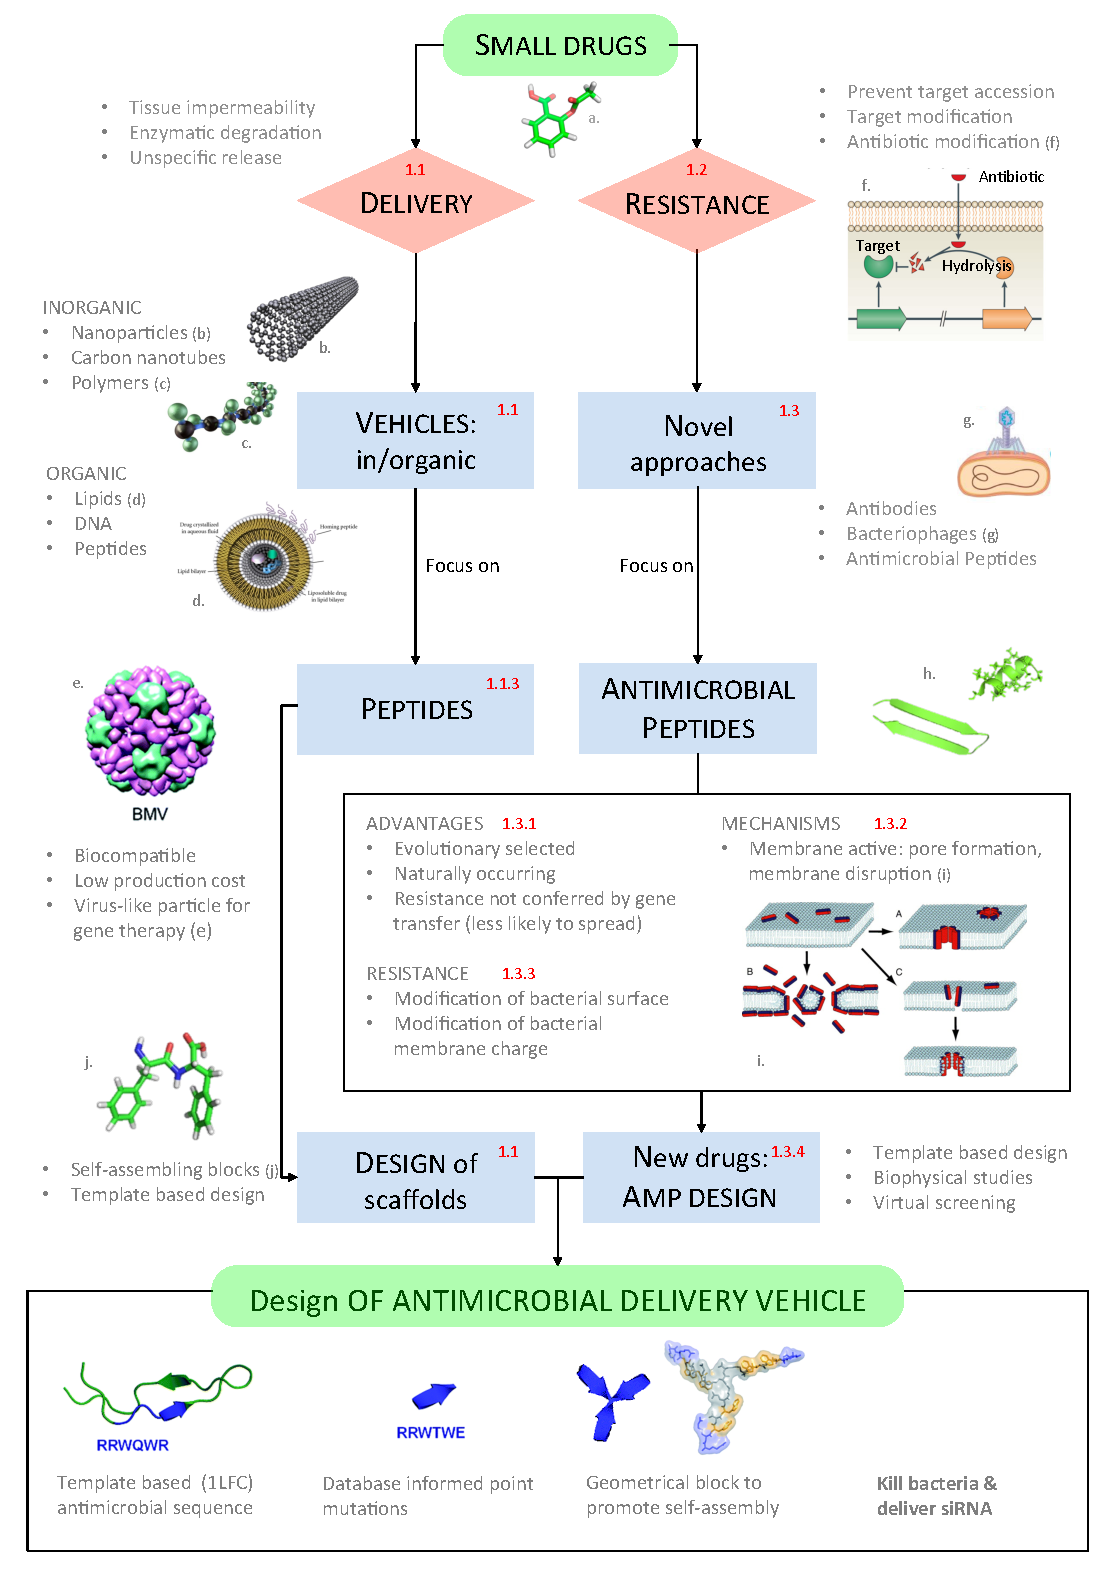
\includegraphics[width = 0.95\textwidth]{1introduction/pics/scheme_intro}
\caption[Graphical abstract of introduction]{Figures a. Acetylsalicylic acid and j. Diphenyl-alanine in bond representation. Remaining figures adapted from: b. \citep{Blair2014}; c. \citep{phage}; d. \citep{Torres2019}; e.\citep{Nguyen2011}; f. \citep{nanotube}; g. \citep{poly}; h. \citep{lipo}; i. \citep{Schoonen2014}; k. \citep{Castelletto2016}; l. in house data.} \label{fig:intro}
\end{center}
\end{figure}

%\clearpage

\section{Antimicrobial resistance}

For most of the last century, the development of new drugs rotated around the paradigm that a drug is a small inorganic compound (of mass up to 900 Da), which intervenes on a specific target of a mammal or bacterial cell. Very often the targets of interest are (intracellular) proteins: out of the 695 small drugs approved by FDA (the American Food and Drug Administration agency) to target human molecules, 667 acts on proteins. Similarly, 189 of the 198 approved to treat pathogens have a protein as their target
%
(with all the caveats coming from the challenges of identifying an unambiguous target, especially when the drug binds to a protein complex or to a number of closely related gene products \citep{Santos2017}).

In presenting the aforementioned figures, the data were naturally split among the drugs which act on human molecules, ``repairing" some faulty process in the human body, or the ones active against bacteria (commonly named as antibiotics) which ``disrupt" the bacterium life cycle in order to kill or prevent the reproduction of the pathogen.
%
It appears evident that the pool of drugs available to the second purpose are in substantially lower number than the ones addressing human molecules. This comes from the nature of the action they perform: molecules targeting human proteins need to be highly specific to avoid interference with other proteins or with healthy cells, and in a sufficient number to address the variety of diseases affecting the human body.
%
Antibiotic must be non-toxic for human cells as well, i.e.\ their target must not be shared between mammal and bacterial cells, but there is a less stringent requirement on their selectivity against different bacterial species. On the contrary, it is often useful to have a broad-spectrum compound. This cross-species efficacy and at the same time non-toxic property is obtained thanks to the evolutionary relationship among bacterial species, and between bacteria and humans: while the first are closely related, and therefore share homologous proteins with very similar structures, humans have less folds in common with them, allowing for a resilience against bacteria-targeting drugs.
%
To be precise, the set of bacterial species is very diverse and the cross-species effectiveness of some drugs does not extend to the whole bacterial population. This is actually demonstrated to be a positive feature, given the large amount of beneficial bacteria that live in symbiosis with the human body (especially in the gut) and that must be preserved for an optimal wellness.

In the framework described above, it is understandable that first-time research on antibiotics was satisfied with the development of a handful of potent, broad-spectrum compounds.
%
Penicillin, the first of them to be synthetically produced, was isolated from a mould in 1928 by Alexander Fleming. It acts inhibiting the formation of a cross-links between particular molecules (peptidoglycan) in the bacterial cell wall, binding to the enzyme responsible for its catalysis, and thus preventing the wall complete formation \citep{Gordon2000} (for further details on bacterial cell membrane structure see Section \ref{sec:host-defense-peptides}).
%
As foreseen from Fleming himself in his Nobel Prize acceptance speech, some species of bacteria quickly became immune to penicillin, and this was achieved in many ways: either by production of penicillase, an enzyme that degrades penicillin, or by subtle changes in the structure of the penicillin-binding proteins to prevent penicillin binding, or again by removal of the drug outside of the cell through specially re-purposed efflux pumps \citep{Lobanovska2017}.

The mechanisms just outlined are not an exceptional characteristic of penicillin, and many drugs lost their effectiveness against some bacteria since their discovery till nowadays, urging the research of new ones on a constant basis. By now, a broad knowledge has been gathered on how bacteria escape the action of a drug: this understanding helps interpreting the pitfalls of existing drugs and identifying the characteristics sought in the development of new compounds.


\subsection{Mechanisms of antimicrobial resistance to small drugs} \label{sec:AMR_mechs}
Antimicrobial resistance can manifest through many different mechanisms, which can be grouped in three main classes, in line with the three processes mentioned in the example of the penicillin resistant bacteria.

\begin{figure}[h]
\begin{center}
\subbottom[]{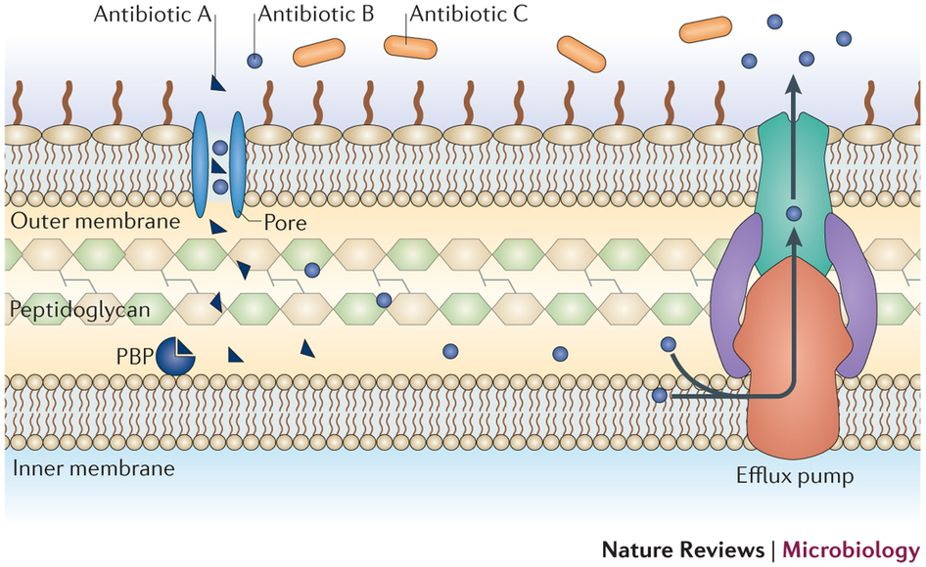
\includegraphics[width=0.6\linewidth]{1introduction/pics/amr1} \label{fig:amr1}} \\
\subbottom[]{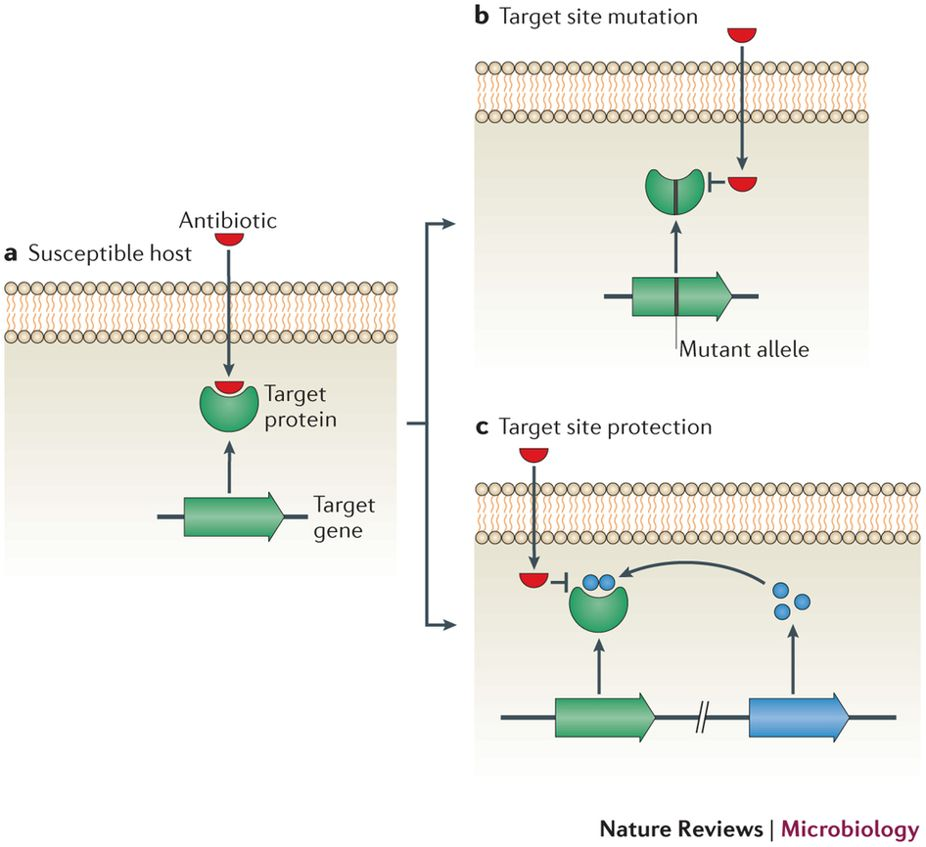
\includegraphics[height = 0.36\textheight]{1introduction/pics/amr3} \label{fig:amr2}}
\hspace{0.5cm}
\subbottom[]{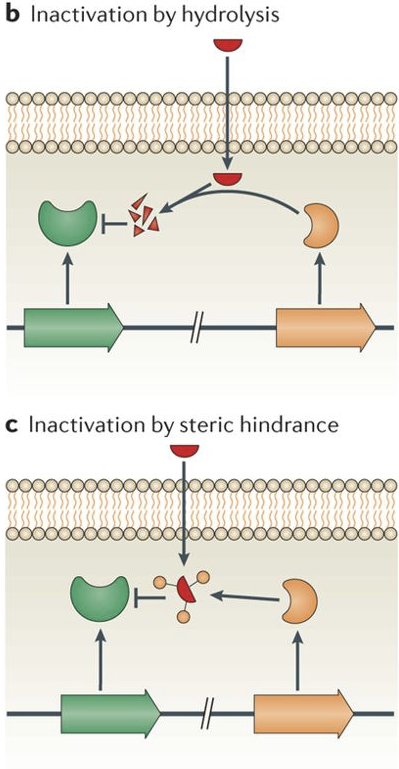
\includegraphics[height = 0.36\textheight]{1introduction/pics/amr4_half} \label{fig:amr3}}
\caption[Mechanisms of antimicrobial resistance to small drugs]{Mechanisms of antimicrobial resistance to small drugs. (a) Intrinsic mechanisms of resistance (removal of antibiotic B by efflux pump and inaccessibility of antibiotic C to the Penicillin Binding Protein target because of membrane impermeability). (b) Target site change via mutation or protection. (c) Direct interactions with antibiotics causing its disruption or structural modification. Reproduced from \citet{Blair2014}.} \label{fig:amr}
\end{center}
\end{figure}

\paragraph{Prevention of access to target}
A first class of resistance mechanisms aims at minimising the intracellular concentration of the antibiotic preventing its penetration or maximising its efflux in the eventuality it has entered the cell (Figure \ref{fig:amr1}).
%
Not all the molecules can enter the cell permeating the membrane, and this holds particularly for hydrophilic antibiotics tackling Gram-negative bacteria which are intrinsically less permeable that Gram-positive ones because of the additional presence of the outer membrane \citep{Delcour2009} (see Section \ref{sec:host-defense-peptides}).
%
These molecules must then be imported into the cell through outer-membrane porin proteins \citep{Vargiu2012,Kojima2013}. Resistance arise when porins are either replaced with more selective channels, which prevent the antibiotic penetration, or down regulated so that the internal concentration of the drug does not reach a critical concentration \citep{Lavigne2013}. Porin-coding genes can also accumulate multiple mutations, to acquire the selectivity they lack in their wild type \citep{Poulou2013}.

A complementary strategy to prevent drug influx is to employ bacterial efflux pumps. Some of them are denominated multidrug resistance (MDR) efflux pumps for their effectiveness in the task and are produced by many bacteria \citep{Floyd2010,Ogawa2012}, but, additionally, can be transferred via plasmids to other bacterial species \citep{Dolejska2013}. Indeed, bacteria are able to exchange genetic material with other individuals via small rings of DNA in a process called conjugation \citep{Sorensen2005}, so that the advantageous resistant genotypes can spread quickly across species.
%
Over-expression of such efflux pump is observed in multidrug-resistant bacteria, triggered by exposition to the drug, and proceeding via mutation in the relative regulatory network, \citep{Abouzeed2008}, or simply as a response to environmental signals \citep{Nikaido2011}.


\paragraph{Change or modification of the antibiotic target}
The second class of resistance mechanisms works modifying the antibiotic target: most antibiotics bind to their substrate with high affinity and specificity, thus small modifications in the target structure can disrupt an efficient binding, still allowing the target to maintain its normal function (Figure \ref{fig:amr2}).

Mutations of some residues in the binding pocket (upon mutation in the gene coding for it) or its post-translational protection via addition of chemical groups are equally wide spread mechanisms.
%
Notable examples of the first include the development of methicillin (an antibiotic in the penicillin class) resistant strains of S. aureus \citep{Shore2011,Billal2011}. Again, it is interesting to notice that several of these mutations are acquired by horizontal gene transfer from other bacterial species, so that resistance development in one specie promotes quickly its insurgence in other ones.
%
For the second process, the most relevant mechanism of chemical group addition is methylation, which, for example, is very common when the drug target are rRNA subunits \citep{Long2006}).


\paragraph{Direct modification of antibiotics}
Finally, bacteria can destroy drugs, usually by hydrolysis, or modify them by transfer of a chemical group (Figure \ref{fig:amr3}).
%
The first historical discovery of drug-degrading enzyme is penicillinase (a $\beta$-lactamase) which destroys penicillin \citep{Abraham1988,Lobanovska2017}. Since then, thousands of similar enzymes have been identified that can modify antibiotics of different classes \citep{Livermore2008,Nordmann2011}:
%
these enzymes co-evolves with newly developed drugs, to include in their spectrum of action new compounds of composition similar to the ones they were originally effective on \citep{Woodford2013}.

Antibiotics constituted by large molecules with many exposed hydroxyl and amide groups are instead particularly susceptible to addition of chemical groups. Many enzymes are responsible for this, and according to the chemical moiety added they are grouped in acetyltransferases, phosphotransferases and nucleotidyltransferases \citep{Wright2005}.

\hspace{0.5cm}
\\
All together, the recent progress in understanding the mechanisms of antimicrobial resistance has helped in directing the development of new drugs, in particular the modification and the improvement of existing compounds to escape the resistance developed by bacteria. To ultimately employ the existing drugs at best, it is important to understand also the dynamics of AMR, beyond its molecular mechanisms, to device the most effective strategies of drug administration.


\subsection{Course of antimicrobial resistance} \label{sec:course_AMR}
In the first stages of the insurgence of antimicrobial resistance (AMR) against a given drug, given strains of bacteria are not damaged by the standard doses of the drug as they came to possess some natural occurring mutations in their genome which promote an escape mechanism invalidating the drug effectiveness \citep{Kapoor2017,Blair2014}. Usually, only a small population of bacteria is resistant in the first instance, however the resistant population will replicate faster that the peers of the same species because it is more fit in an environment challenged by the presence of the drug. It is noteworthy that this fitness might not be optimal in a natural drug-free environment, and indeed the wild population has not been selected for that genotype.
%
To prevent this insurgence, high doses are often used, to kill the bacteria in a short time and decreases the chances of resistance development \citep{Baker2018}. However, high drug doses are not always applicable due to the severe side effects they are connected to, creating favourable conditions for resistant strains.

As already mentioned, the spread of resistance between bacterial cells and even between species is very effective as bacteria exchange genetic material through conjugation.
%
Therefore, despite AMR is an evolutionary mechanism, the fast pace at which bacteria replicates, their enormous population (in terms of individuals), and the relative easy horizontal gene transfer, place the insurgence of resistance well within the human lifespan time scale \citep{Oneill2016}.

It is then clear that this complex problem depends on many variables: the casual appearance of resistant individuals, the transfer of information between them, the relative gain in fitness that the mutation implies, but also the dosage and time line of the drug administration. Many mathematical models have been implemented to understand the issue \citep{Birkegard2018,Niewiadomska2019}, and it is known that some strategies of drug administration are actually promoting the proliferation of so called ``super" bugs.
%
One example is the underdosage of antibiotics which is likely to harm but not to kill pathogens, rather promoting the fitness of resistant ones, or their abuse, as it puts an high pressure on the pathogenic populations, which is desirable but can sometimes induce a faster emergence of escape mechanisms \citep{Oneill2016}.

In this context it must be noticed that many drugs are bacteriostatic agents as opposed to bactericidal: i.e.\ they prevent the bacterium growth rather than kill it, as they are meant to slow down the damage while host defence mechanisms eradicate them.
%
Thus if an high dosage of a bactericidal agent may extinguish the bacterial population and eradicate the disease, bacteriostatic drugs allow bacteria to start again the reproduction cycle once removed (if the host defence could not properly work).

It is then clear that the antibiotic landscape is dynamically regulated: newly discovered drugs enter, while others exit after having been exploited for years, therefore we need constant input from research to find new treatments to old diseases. The severity of the AMR treat is such that it has been raised to the status of national emergency in several countries, including UK. Indeed, strict regulations on the health, agricultural and food industry sector must be taken to prevent the misuse of antibiotics, as we are leaving the century in which antibiotics were discovered, to enter a phase in which we count the number of the ones loosing efficacy \citep{Oneill2016}.


\section{Alternative antibiotic strategies: antimicrobial peptides}
In the landscape sketched above, it is evident that the development of novel drugs is of crucial importance. Even more beneficial would be to have at disposal a new paradigm for their design, in order to attack pathogens in a completely novel way, avoiding to target pathways which are known to lead easily to the development of antimicrobial resistance. Several novel materials have been developed for the task, not to rely on small molecules and exploit different mechanisms of action, for example antibodies, bacteriophages or antimicrobial peptides \citep{Mantravadi2019}.

While the use of pathogen-specific antibodies relies on mechanisms of the host immune system, bacteriophages therapy employs viruses which infect bacteria and archea rather than eukarya.
%
But antimicrobial peptides are the main focus of this thesis: indeed some peptides can have an active role against bacteria, if their sequence possesses specific characteristics, and are thus referred to as antimicrobial peptides. The following subsections will explore their characteristics, modes of action and the response of bacteria against them. It is indeed crucial to understand the knowledge available versus the questions that are still open in order to direct the efforts of future research. This holds in particular when the investigation proceeds by the use of simplified models, as the ones employed in Computational Biology, as meaningful results can proceed only if such modelling is performed in a sensible and informed fashion.

\begin{figure}
\begin{center}
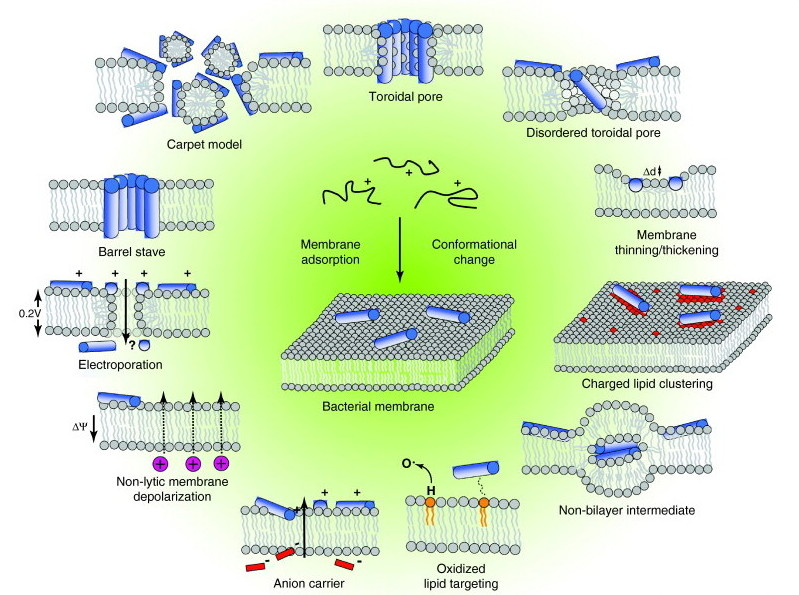
\includegraphics[width = 0.8\textwidth]{1introduction/pics/amp_mech.jpg}
\caption[Modes of action of antimicrobial peptides]{Events occurring at the bacterial cytoplasmic membrane following initial antimicrobial peptide (AMP) adsorption. Reproduced from \citet{Nguyen2011}.} \label{fig:amp}
\end{center}
\end{figure}


\subsection{Membrane active peptides} \label{sec:host-defense-peptides}
Antimicrobial peptides (AMPs) are naturally produced by eukarya, either as stand-alone sequences or embedded in larger proteins, as a first, weak, and broad-spectrum defence against bacteria \citep{Nguyen2011}.
%
This pool of molecules has been selected though evolution to be active against pathogens, suggesting that they will most likely not cause resistance in the near future.

To exploit their potential and engineer AMP-like molecules, a careful characterisation and classification of such peptides must be done. This task has been carried on throughout the past decades but because of its complexity at present there are many peptides with ascertained antimicrobial activity for which the mode of action is still not fully understood \citep{Ebbensgaard2015}. However, some general characteristics of these sequences and some of the mechanisms they employ have emerged.
%
Unsurprisingly, AMPs are heterogeneous in  sequence, structure, targets and modes of action, to tackle the different challenges bacteria pose. Their size can vary between 6 and 59 amino acids \citep{Brogden2005}: despite being small with respect to the average size of a protein in the human body, these macromolecules are hundreds of times larger than small molecule drugs and as such they penetrate and act on bacteria differently with respect to small compounds.

The most common target of AMPs is the bacterial membrane. Many of them cause disruption of the physical integrity of the microbial membrane while others translocate into the cytoplasm to act on intracellular targets, and the combination of the two is not uncommon either \citep{Hancock2006} (Figure \ref{fig:amp}). In general, it is widely accepted that membrane interaction and its relative consequences are a key factor for the antimicrobial activity of AMPs \citep{Nguyen2011}.

As such, we propose a brief overview of the structure of the bacterial membrane \citep{Silhavy2010}, and of its differences with the one of mammalian cells, to better understand how AMPs can be effective and selective against bacteria at once.


\paragraph{Structure of bacterial membrane}
The determinant driving the interaction between AMPs and bacterial membranes is the positive charge that many AMPs present, opposed to the negative charge of the latter \citep{Nguyen2011,Mahlapuu2016}.
%
It is striking that such simple mechanism, based on the presence of a certain number of negatively charged lipids, holds across many bacterial species despite the great variability found in their membrane composition.
%
Indeed, based on the differences in their cell envelope structure, bacteria are classified into two macro families, Gram-positive and Gram-negative.
%
In Gram-positive bacteria, the cytoplasmic membrane is surrounded by a thick peptidoglycan layer, while for Gram-negative bacteria this membrane (which assumes the name of internal one) is surrounded by a thin peptidoglycan layer as well as an outer membrane \citep{Silhavy2010,Lin2016} (Figure \ref{fig:membranes}).

\begin{figure}[t!]
\begin{center}
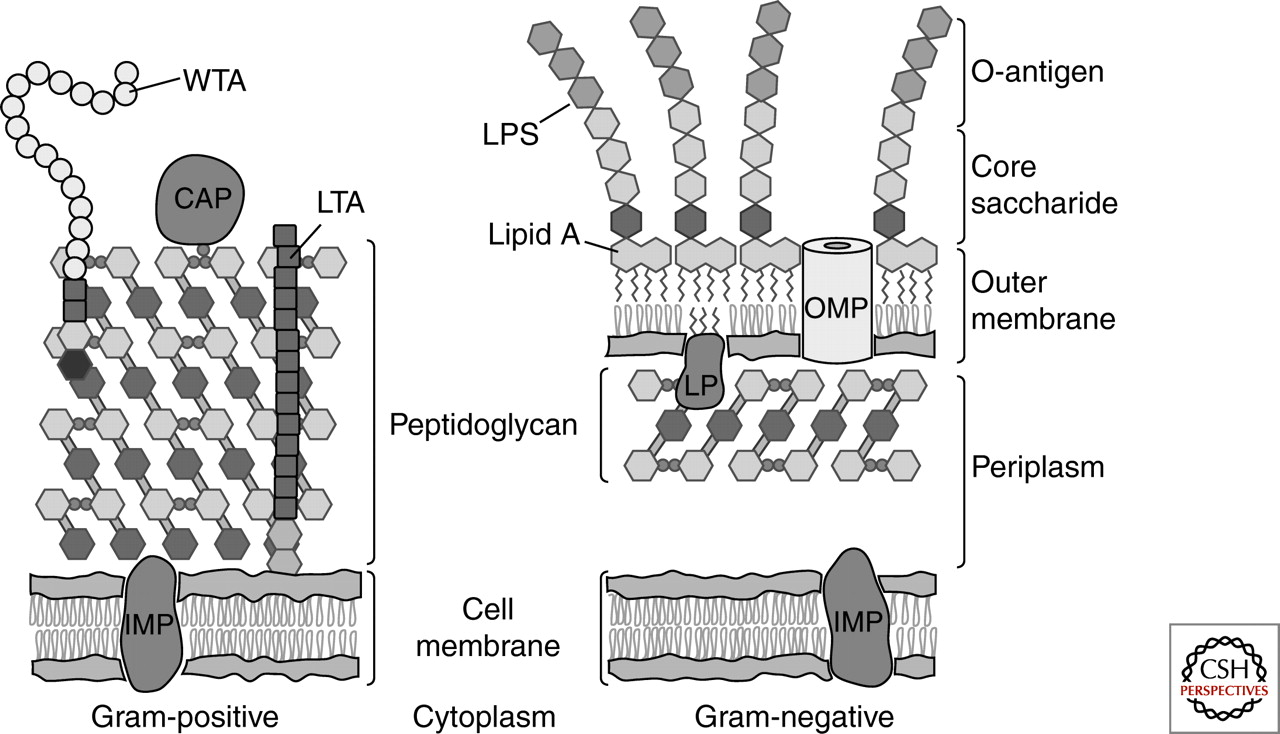
\includegraphics[width = 0.8\textwidth]{1introduction/pics/bacterial_membrane.jpg}
\caption[Structure of Gram-positive and -negative cell envelope.]{Structure of Gram-positive and -negative cell envelope. IMP: integral membrane protein; CAP: covalently attached protein; LTA: lipoteichoic acid; WTA: wall teichoic acid; LP: lipoprotein; OMP: outer membrane protein; LPS: lipopolysaccharide. Reproduced from \citet{Silhavy2010}.} \label{fig:membranes}
\end{center}
\end{figure}

Starting from the inside and proceeding outwards (from bottom to top of Figure \ref{fig:membranes}), the cytoplasmic membranes of both Gram-positive and Gram-negative bacteria are rich in phospholipids like phosphatidylethanolamine, which is neutral, and phosphatidylglycerol, cardiolipin, and phosphatidylserine, which have negatively charged headgroups, highly attractive for positively charged AMPs \citep{Silhavy2010,Lin2016}. This is often sufficient to promote the preferential interaction between this membrane and the peptides - provided they get into its proximity.
%
Perturbation of this membrane is highly disruptive as many functions are associated to it: as bacteria do not possess organelles, all the membrane-related proteins reside and perform their function within the inner membrane.

In the case of Gram-negative bacteria (Figure \ref{fig:membranes}, right), the inner membrane, together with the outer one, delimits the periplasm space, an aqueous cellular compartment, which allows the sequestration of harmful substances and the transport of nutrients.
%
Proceeding outward, inside the periplasm is situated the peptidoglycan cell wall. This substance is made of a disaccharide cross-linked by penta-peptide side chains (from which the name), and these repeated units constitute the rigid skeleton of Gram-negative bacterial cells \citep{Gan2008}. It is fundamental for cell life as damage in the peptidoglycan layer results usually in living but not viable cells \citep{Joseleau-Petit2007}.

Grafted to the cell wall through Braun’s lipoproteins (or LPP) \citep{Asmar2018} is the outer membrane. This membrane presents an asymmetric structure: phospholipids are present in the inner leaflet, while the outer one is composed of glycolipids, mainly lipopolysaccharides (LPS) \citep{Silhavy2010}. These complex molecules consist of lipid A, which presents multiple fatty acids, and a polysaccharide \citep{Raetz2002}. The polysaccharide is made of an inner core, covalently bond to the lipid, an outer core, and finally a repetitive glycan polymer (O-antigen). The O-antigen (top right in Figure \ref{fig:membranes}) is the molecule exposed by Gram-negative bacteria to the external environment and thus is the target of antibodies recognition.

Given the complexity of the Gram-negative cell envelope, and especially the presence of the LPS layer, these bacteria are particularly impermeable to hydrophilic molecules, which are usually imported within the cell through porins and similar transmembrane proteins.

For Gram-positive bacteria (Figure \ref{fig:membranes}, left) the inner membrane is enveloped in a thick peptidoglycan layer. If its thickness in Gram-negative bacteria reaches few nanometers, in Gram-positive ones it spans from 30 to 100 nm. Its composition is similar to the one described above, with some variations present among different bacteria, for example in the nature of the peptidic linker or in its precise position \citep{Vollmer2008}. This thick layer is threaded by long anionic polymers (the teichoic acids), mainly composed by glycerol phosphate, glucosyl phosphate, or ribitol phosphate repeats \citep{Swoboda2009}. Disseminated in this layer there are several surface proteins with various functions, among which adhesins, which attach to components of the host extracellular matrix.

Gram-positive membranes are generally more permeable because they do not possess a double-membrane structure, nevertheless the peptidoglycan later they are coated with constitute a challenge for drug delivery.


\paragraph{Comparison with mammalian membrane}
The fact that AMPs tackle negatively charged membranes is crucial for their selectivity, i.e.\ that they are harmless for the mammalian cells they are produced from \citep{Glukhov2005}. This is possible because mammalian cells have a different membrane composition. They present a single membrane, which is rich in proteins (up to 50\% of its volume) and in lipids, with a small percentage of carbohydrates, mainly embedded in glycoproteins, which promote cell-cell recognition.

The lipidic component is abundant in zwitterionic phospholipids such as phosphatidylethanolamine, phosphatidylcholine, and sphingomyelin, providing a neutral net charge. \citep{Spector1985,vanMeer2008}.
%
Furthermore, the mammalian cell membrane has a high content of cholesterol \citep{Yeaman2003, Lai2009}, a sterol fat, which is proposed to stabilise the membrane regulating its fluidity across the differences of physiological temperatures, and it is also though to favour a better accommodation of the perturbations caused by AMPs \citep{Zasloff2002}.
%
Strictly speaking, some negatively charged lipids are present in a few mammal cell types, however they are located in the inner leaflet, while the zwitterionic phospholipids are more abundant in the outer leaflet, in an asymmetric composition \citep{vanMeer2008,Matsuzaki2009}.
%
This structure promotes weaker interactions between AMPs and mammalian cells with respect to bacterial ones, as the former is driven mainly by hydrophobic interactions, while the latter by electrostatic ones.

Another relevant difference between bacterial and mammalian cells is that the first ones have typically a higher transmembrane potential - the difference of electrostatic potential between the inside and the outside environment: for bacteria it falls between $-130$ and $-150$ mV, while for mammalian cells between $-90$ and $-110$ mV \citep{Yeaman2003,Matsuzaki2009,Ebenhan2014}.
%
Given that a potential generates an electric field across the membrane, the higher this is, the higher the resulting electric field pointing from outside to inside the cell will be. A field in such direction pushes cationic compounds on the outside of the membrane toward the membrane itself. Therefore the stronger bacterial transmembrane potential may promote an enhanced - and thus disruptive - interaction of AMPs with the cell, contributing to the AMPs selectivity between bacteria versus mammals \citep{Yeaman2003}.


\subsection{Common mechanisms of action of AMPs} \label{AMP_mechs}
Investigating the perturbation and disruption of a bacterial membrane by antimicrobial peptides is a key point of this work, therefore it is important to highlight the mechanisms known so far through which AMPs reach this outcome.
%
As already mentioned, many AMPs have a positive charge which facilitates the binding to the membrane via charge-charge recognition; accordingly, Arginine and Lysine residues are usually abundant in AMPs sequences. However, the disruptive action takes place through the interaction of the AMP with the hydrophobic core of the membrane, therefore their sequences contain also hydrophobic aromatic residues, especially Tryptophan, which favours the anchoring to the lipid core \citep{Chan2006}.
%
Overall, AMPs resort often to adopt an amphiphatic structure to segregate the hydrophilic from the hydrophobic amino acids and thus act at the interface between membrane and solution. It is interesting to notice that some of them fold into the active structure only in the nearby of the membrane, as they can expose their hydrophobic components to face its core, while in solution these ones are preferentially buried inside to be screened from the solvent \citep{Nguyen2011}.
%
Common folds adopted by AMPs are both $\alpha$-helix or $\beta$-sheet rich structures. Amphiphatic $\alpha$-helices present a charged side which is tailored to face towards the phospholipid head groups and an hydrophobic ones which is favourably buried into the acyl chains core,
%
and a similar arrangement is found for structures rich in $\beta$-sheets include $\beta$-hairpins (Figure \ref{fig:amp_structure}).


\begin{figure}[t!]
\begin{center}
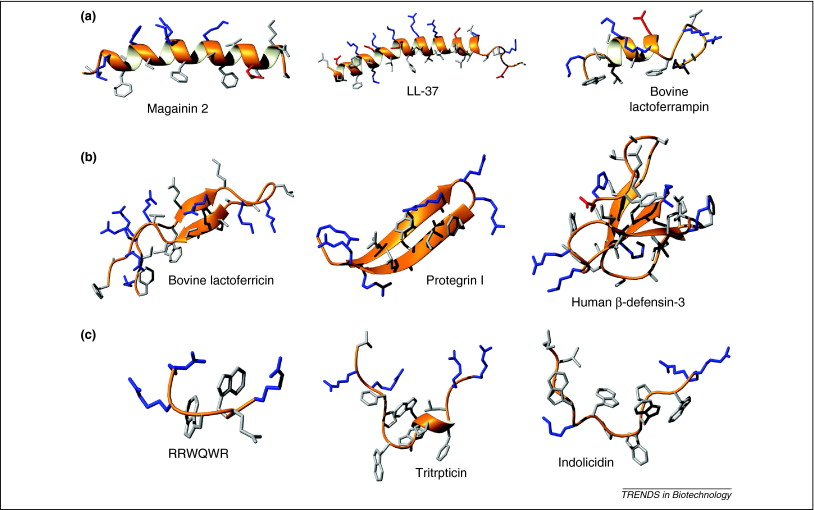
\includegraphics[width = 0.8\textwidth]{1introduction/pics/AMP_many.jpg}
\caption[Structure of some known AMPs.]{Structure of some known AMPs. Reproduced from \citep{Nguyen2011}.} \label{fig:amp_structure}
\end{center}
\end{figure}


\paragraph{Membrane disruption} Several models have been proposed to describe the exact mechanisms of AMPs penetration after they bind to the cytoplasmatic membrane, and how their combined action leads to membrane permeabilization (Figure \ref{fig:amp}) \citep{Brogden2005,Nguyen2011}.

For example, for a single copy of a amphiphatic helical AMP, the proposed mechanism of action suggests that initially the peptide is attracted with its charged side to the membrane and lies parallel to its plane, with the hydrophobic side unfavourably exposed in solution. Then the helix rearranges to have the two faces in the respective favourable regions. Subsequently, the helix axis starts to form an angle with the membrane plane, and finally inserts deeper into the lipid core, often spanning the full membrane thickness \citep{Ebenhan2014}.
%
Similarly, for $\beta$-sheet rich structures, it is suggested that they insert within the membrane after a first flat approach.
%
The final insertion arrangement depends on the peptide characteristics and length, the presence of kinks in its structure (in case of helices), and the interactions with other copies of the peptide.

The picture becomes more complex for oligomer-mediated insertion, i.e.\ when the action is triggered by the combined action of many copies of the peptide.
%
At low peptide to lipid ratio, the favourable configuration is represented by peptides lying parallel to the membrane plane as described previously \citep{Yang2001}, but an increase in peptide concentration triggers the transition to an inserted state where the main axis of the AMP is perpendicular to the membrane. The organisation of AMPs inside the membrane core can assume different configurations, as described below \citep{Brogden2005,Nguyen2011,Ebenhan2014,Mahlapuu2016} (see Figure \ref{fig:amp}).

The ``barrel-stave" model proposes that AMPs insert perpendicularly into the bilayer.
Recruitment of peptides in the same area results in the formation of a transmembrane pore with a central lumen. The walls of the pore are constituted by the hydrophilic face of the peptides, while their hydrophobic side is interacting with the lipid tails around the pore. This model is adopted for example by the $\alpha$-helical AMP alamethicin, which forms voltage-dependent ion channels by aggregation of four to six molecules \citep{Spaar2004}.

In the ``toroidal" pore model instead, the insertion of peptides forces the phospholipid to bend continuously from one leaflet to the other.
%
The toroidal model differs from the barrel-stave model as the peptides are always associated with the lipid head groups even when they are perpendicularly inserted in the lipid  bilayer. Toroidal pores are induced by $\alpha$-helical magainins, protegrins and melittin \citep{Yang2001,Matsuzaki1996,Hallock2003}, and lead to membrane perturbation which extends further away from the pore than in the barrel-stave case, as lipids must rearrange around them: as a comparison, alamethicin induced barrel-stave pores have an inner and outer diameters of 1.8 nm and 4.0 nm respectively \citep{Spaar2004}, while magainin-induced toroidal pores have variable sizes, with an inner diameter of 3.0-5.0 nm and an outer diameter of 7.0-8.4 nm \citep{Matsuzaki1997}.

Finally, in the ``carpet" model, the accumulation of AMPs on the surface of the membrane, laying parallel to it, causes tension in the bilayer and the membrane is then disrupted by peptides in a detergent-like manner, leading to the formation of micelles.
%
The critical threshold concentration triggers a cascade effect, in which formation of the first disruption allows the penetration of AMPs in the inner side of the bilayer. The cooperation between peptides on both sides of the lipid membrane enhances the AMP-induced curvature causing accelerated disruption.
%
The ``carpet" model mechanism is observed for peptides presenting an $\alpha$-helical structure (like melittin \citep{Ladokhin2001}) or several helices connected by short loops (ovispirin \citep{Yamaguchi2001}).

The prevalence of examples with an helical structure for the above models derives from the fact that the understanding of how helical AMPs function is often easier than the one of $\beta$-sheet rich structures.
%
Indeed, helices have a well defined fold (at least nearby the membrane environment), a compact structure, and often a clear segregation of complementary patches that can attract other copies of the peptide and thus promote the self-assembly process necessary for the pore formation.

On the contrary, many $\beta$-sheet AMPs have a more flexible structure, and more diversified mechanisms of action \citep{Nguyen2011,Mahlapuu2016}.
%
AMPs rich in $\beta$-sheets can be divided into $\beta$-hairpins and peptides from the defensin family \citep{Nguyen2011}.
%
Many representative of the former class disrupt bacterial membranes via formation of toroidal pores: as an example, porcine peptide protegrin I triggers the toroidal pore formation assembling into a $\beta$-barrel structure when in contact with anionic membranes (while it folds into $\beta$-sheet aggregates on the surface of cholesterol containing membranes, thus acting selectivity on bacterial membranes only \citep{Tang2009}).
%
In the case of defensins, many mechanisms are known according to the specific member of the family \citep{Lehrer2004,Kagan1990,Takeuchi2004}.
%
Although various descriptions of membrane damage have been reported, and include ion channels, transmembrane pores and extended rupture of the membrane, they are likely related, being a modulation of a similar acting principle.


\paragraph{Alternative mechanisms of action} Finally, many non-lytic mechanisms are suggested for AMPs, especially for $\beta$-sheet structures: defensin A from P. terramovae reduces the cytoplasmic potassium concentration \citep{Brogden2005}, partially depolarising the inner membrane; tachyplesin from horseshoe crabs is able to bind to the minor groove of DNA, interfering DNA–protein interactions \citep{Yonezawa1992},
%
and bovine lactoferricin can act synergistically with other antimicrobial agents by affecting the transmembrane potential and proton-motive force, resulting in inhibition of ATP-dependent multi-drug efflux pumps \citep{Gifford2005}.
%
Moreover, after translocation within the cell, bovine lactoferricin can also inhibit DNA, RNA and protein synthesis.

Section \ref{sec:capzip} will treat in detail the functioning of this AMP, distinguishing its role as membrane active peptide as opposed to intra-cellular targeting compound: indeed, many works have focussed on lactoferricin antimicrobial processes versus locating the section of the sequence performing the membrane disruptive activity \citep{Tomita1994,Schibli1999}, to understand whether it retains the efficacy regardless of the fold.
%
These type of investigations performed on many AMP sequences provided the discovery of first minimal functioning antimicrobial blocks, which promoted the understanding of how AMPs work in general, and boosted the design of synthetic AMPs tailored for specific functions.


\subsection{Mechanisms of resistance to AMPs}

Antimicrobial peptides were introduced here as a class of new drugs and a possible solution to the crisis of antimicrobial resistance. Any new drug entering the pool of the clinically approved compounds is (at least temporary) a solution to the problem of resistance to known antibiotics; but it must be clarified that bacteria can develop resistance to AMPs too.
%
Nevertheless, the resistance to their action is generally not based on dedicated genes that are conferred by horizontal gene transfer, as in the case of many antibiotics resistance mechanisms \citep{Peschel2006}. Because of that, a certain increase of resistance after exposure to the drug is to be expected, but it is less likely to spread quickly to other species.

Some of the mechanisms of AMPs resistance are similar to the ones employed by bacteria to counteract small molecule drugs, for example over-expression of efflux pumps to dispose of AMPs, degradation of the peptide by extracellular enzymes and sequestration by the bacterial or biofilm matrix to prevent accession to the target \citep{Peschel2006}.

Differently with respect to antibiotics hydrolysis, AMPs proteolitic degradation is operated by proteases, secreted on the extracellular side of the membrane specifically to destroy other proteins. Linear AMP are more prone to this type of degradation \citep{Sieprawska-Lupa2004}, as opposed to the ones presenting disulfide bonds \citep{Peschel2006}, such as defensins, which nevertheless can be hydrolysed by more specific proteases enzymes \citep{Nelson2011}.

Bacteria can also enhance their resistance to AMPs organising into specialised structures known as biofilms \citep{Costerton1999}. Biofilm bacteria adhere to a surface and secrete an extracellular matrix with adhesion and protection functions \citep{Jolivet-Gougeon2014}, which effectively repels and/or captures AMPs.
%
For example the polysaccharide intercellular adhesin (PIA) present in the extracellular matrix of S. aureus and other bacteria can be deacetylated to increases its positive net charge, thus repelling more efficiently cationic AMPs (like HBD-3, LL-37), and increasing sequestration of the anionic ones (like dermcidin) at the same time \citep{Vuong2004,Vuong2004PIA}.
%
AMPs are nevertheless a promising alternatives in the treatment of biofilm-associated infections. In this type of infections bacteria are growing slowly, so it is advantageous to have bactericidal agents such as AMPs, as opposed to bacteriostatic ones such as traditional antibiotics which target fast-growing bacteria only \citep{Strempel2014}.

But the most specific mechanism of AMPs resistance concerns modifications of the bacterial cell envelope: bacteria modify the characteristics of their surface to prevent the efficient binding of an AMP, even in the eventuality that the peptide reaches the bacterial envelope intact. 
%
The target of such modifications are different for Gram-positive and Gram-negative bacteria, according to their distinct cell envelopes.
%
Gram-positive bacteria change the structure of their teichoic acids (TA): for example, D-Alanylation of TA observed in S. Aureus adds a positive charge to it, reducing the attraction of cationic AMPs and in turn increasing the cell wall density, so reducing the surface permeability \citep{Saar-Dover2012}.
%
Alternatively the bacterial peptidoglycan precursor, lipid II, can be modified: it has a key role in the formation of the cell wall ad is often targeted by AMPs. For example, the replacement of its terminal D-alanine with D-lactate or D-serine \citep{Bugg1991} avoids the action of the glycopeptide vancomycin, which binds to the D-Ala-D-Ala terminal motif of the precursor.

In Gram-negative bacteria a positive charge can be added to lipopolysaccharides (LPS) by addition of amine-containing molecules \citep{Moskowitz2004} or by removing phosphate lipids (which have a negative charge) from lipid A \citep{Wang2006lpx}, to obtain the same effects as for the increased charge in TA.
%
Importantly, the resistant Gram-negative bacteria can also enhance the rigidity of the outer membrane to reduce permeability to AMPs via addition of extra acyl chains into lipid A \citep{Guo1998}.
%
Moreover, they can act at the cytoplasmic membrane level, as this is the final target of many antimicrobial peptides: in the eventuality that AMPs successfully reach this membrane, they are attracted to its surface by the negative charge of the lipids composing it, in particular phosphatidyl-glycerol (PG) and diphosphatidylglycerol (DPG, also called cardiolipin). Their negative charge can be masked by amino-acylation of the PG head group, so that the final compound repels AMPs through electrostatic interaction \citep{Peschel2001}; alternatively the overall rigidity of the cytoplasmic membrane can be enhanced, by an increase in saturated acyl chains which has been proven to confer resistance \citep{Kumariya2015}.
%
To be noticed that resistant bacteria often employ many of the aforementioned strategies at the same time \citep{Band2014}.


\subsection{Principles of AMP design} \label{sec:amp_design}

The study and classification of AMPs provide knowledge on the characteristics a sequence must have to perform an antimicrobial function.
%
As discussed in Section \ref{AMP_mechs}, there are some features which, comprehensively, help in discriminating AMPs against non antimicrobial peptides. The constantly increasing amount of data available is gathered in several curated databases \citep{APD3,DBAASP2,dbAMP,antiBP2,amPEP}, which catalogue AMPs (or subclasses of them, like membrane active, biofilm active or haemolytic peptides) based on such features to promote future data-driven prediction of the antimicrobial character of a sequence.

We recapitulate below a few key characteristics which are peculiar of AMPs. To be noticed that while some are easily retrievable from the sequence of the peptide, others imply direct experimental measures:
\begin{itemize}
\item \textbf{Structure}: both $\alpha$-helical and $\beta$-sheet rich AMPs exist, as well as mixed structures. Short helix ($\sim$ 22 amino acids) and short $\beta$-sheet ($\sim$ 10 amino acids) are particularly common. When screening a potential AMPs, it must be considered that the fold adopted by the peptide close to the membrane environment might be different with respect to the one in solution.
%
\item \textbf{Charge}: AMPs are charged moieties, usually cationic (up to $\sim + 10\,e$), with fewer anionic examples (like dermcidin). Among cationic ones, not all the positive amino acids have equal role, for example Arginines are more effective than Lysins \citep{Chan2006}. The potency, but also their haemolytic activity, are often directly related to the amount of charge \citep{Jiang2011}.
%
\item \textbf{Hydrophobicity}: AMPs contain also hydrophobic residues, usually with abundance of aromatic chains and specifically Tryptophan, as they must insert and anchor into the lipid core of membranes, which is an hydrophobic environment.
%
\item \textbf{Amphipathicity}: to host both the charged and hydrophobic residues, most AMPs organise themselves in an amphiphatic structure, i.e. the two types of amino acids side chains are located on the opposite sides of the peptide.
%
\item \textbf{Solubility} AMPs need good solubility to prevent aggregation in the aqueous environment they float in before arriving to the membrane. Aggregation would most likely impede their optimal interaction with the membrane.
\end{itemize}

A part from predictions regarding existing sequences, the knowledge of AMPs sequence-activity and structure-activity relationships is beneficial to find new, better performing ones. The design of new AMP sequences aims at producing peptides with improved characteristics:
\begin{itemize}
\item \textbf{specificity} against particular bacterial species;
\item \textbf{stability} against the action of proteases, thus allowing a longer residence time in the body;
\item \textbf{low cytotoxicity} at the therapeutic dose required (so an high therapeutic index).
\end{itemize}
The need for such improved peptides lies in the fact that their natural form constitutes a first broad spectrum defence our body employs against infectious bacteria and thus AMPs are often of mild potency. However, foreseeing their application as future drugs, it is desirable to tailor them to fulfil different criteria according to the infection to treat.
%
At the present state of the art, a golden rule for the design of such sequences is still missing, however several methodological approaches to AMP design have been explored, and they can be grouped in three main lines: template based studies, biophysical studies and virtual screenings \citep{Fjell2011}.

\paragraph{Template based studies}
The main idea behind template based methods consists in modifying existing antimicrobial sequences in the direction of the desired characteristics. The most widely explored templates are helical peptides, for their short sequences and because several of them (cecropin, magainin and protegrin) have been well characterised \citep{Wang2015}.

Ideally, an amino acid scanning of all the residues in an AMP provides information on the role of each of them, prompting at the most suitable mutations. High-throughput methods for the synthesis and characterisation allow nowadays for such thorough investigation in the case of short AMPs \citep{Hilpert2005}, but similar, less resource consuming Alanine scannings can still point at the most important residues for the antimicrobial activity \citep{Migon2018}.
%
Alternatively, simpler approaches aim at designing peptides with enhanced charge and amphiphilicity, as these characteristics are deemed crucial for their effectiveness (see the paragraph above) \citep{Wang2015}.

However, all the above methods focus on single amino acids and can not take into account the interplay between residues, nor the three dimensional structure of the peptide. Without such information, it is difficult to extract general rules on why some mutations work better, and often the results of these studies give indeed enhanced AMPs, but cannot be generalised to other sequences.
%
Therefore, recent works sought to integrate structural information on template based models, successfully designing peptides active against many bacterial lines at the same time \citep{Liu2018} or enhancing the selectivity of some sequences for bacterial membranes \citep{Jiang2011}.

A complementary approach to single point mutations on known peptides consists in designing minimal antimicrobial blocks: several investigations proved the importance of single residues and their intercalated pattern in natural and designed AMPs. For example, natural AMPs are rich in Tryptophan and Arginine residues \citep{Chan2006}, and synthetic ones have been produced with only Lysines-Leucine, or Arginine-Valine combinations to produce amphipathic helices \citep{Deslouches2005}.
%
An effort to extract principles from these examples is represented by text based models where amino acids constitute the letters and patterns occurring in natural AMPs are the grammar rules \citep{Loose2006,Cipcigan2018,Spanig2019}.

In general, the advantage of template based methods is in the reduced number of sequences to test, with decreased cost, as only a subspace of them is explored, namely the ones close to the original template.


\paragraph{Biophysical studies}
Biophysical studies aim at understanding the functioning of AMPs investigating their structure. Free energy perturbation, Molecular Dynamics (MD) simulations and thermodynamics calculations can all provide knowledge on how the three dimensional arrangement of residues is important to allow their functional role.
%
Contrary to sequence based methods, these techniques give an insight into the mechanism of action of an AMP but their drawback lays in the high computational cost. For example simulations can approach systems with a limited size, and only on short (microseconds) time scales, preventing the reproduction of phenomena of the order of millisecond (a detailed overview of the state of the art, advantages and drawback of MD simulations will be given in Chapter \ref{chapter:MD}).
%
For these reasons, such techniques have been applied to fewer systems in comparison to sequence based screenings, and only few mutations have been tested and compared \emph{in silico}.

The strength of biophysical studies lay instead in the fact that they exploit the whole information available on a system (sequence, structure, chemistry), so they can single out the interactions that are crucial for a mechanism, clarifying whether they can be transferred to a different environment, or again they can discriminate cases in which similar sequences behave differently due to the environment around them. In this respect, they provide a generalisable knowledge applicable to different systems and thus to the design of novel AMPs at the atomistic level. Extensive examples of such workflow are given in Section \ref{sec:md_lit}.

\paragraph{Virtual screenings}
Contrary to biophysical assays, virtual screening methods are employed to analyse a large number of sequences, when an experimental or computational test of all of them would be prohibitive. The concept of these methods consists in identifying descriptors which allow to predict the potency of the sequence: from the analysis of a database of AMP with known activity, a model is created and used to score novel synthetic sequences \citep{Fjell2011,Kleandrova2016}.

The recent evolution of machine learning (ML) techniques, artificial neural network in particular, gave a great impulse to virtual screening of AMPs (for a historically informed review see Table 1 in Ref. \citep{Fjell2011,Veltri2018}). Machine learning appears particularly suitable to the task as the potency of AMPs is determined by the combination of many factors, the relative weight of which can be difficult to identify. Moreover, these approaches can help in the identification of relevant features traditionally overlooked.

Practically, ML algorithms are trained on a set of AMPs labelled by their potency and characterised by different properties (features) along the line of the ones mentioned at the beginning of the section: sequence, partial charge, hydrophobicity, etc; but also experimental measures (pK measures, nuclear magnetic resonance data, octanol-water partition fraction and so on).
%
The more the input properties to consider, the more expensive is to train the model, but the higher the accuracy that can be meet. At the same time, the output descriptor is increasingly complex (i.e.\ a combinations of many features) and thus of difficult interpretation.
%
In principle, this is not a problem (provided there is no overfitting) as, rather than guide the design of AMPs from first principles, descriptors can be used to score combinatorial sequences of the desired length to identify the best ones. In practice however this is often difficult because of their exponentially growing number.

The second obstacle to ML procedures is given by the fact that the more features one wants to consider, the more sequences need to be given as input to the algorithm, i.e.\ need to be experimentally tested.
%
However, modern high-throughput synthesis methods, together with surrogate measures of bacterial killing are allowing it nowadays, as shown by \citet{Cherkasov2009}, who assessed the antimicrobial properties of thousands of 9 residues sequences and trained a neural network on the outcome, to then score novel sequences with good accuracy. This is a first step toward an automated and general procedure for AMP design.

\subsection{Clinical applications}
Antimicrobial peptides have been studied for many years, however the push to capitalise them to get compounds viable for the clinical stage has been delayed by many factors, including production costs, and lack of interest in the face of more potent small molecules which were deemed more economically advantageous by pharmaceutical companies.
%
The constant increase of AM resistance has resulted in more effort focusing on AMPs, mainly from small biopharmaceutical companies, and at present several of these preparations are in clinical trials, either in phase 1 or 2 \citep{Naafs2018}.

The two major problems encountered so far for AMPs sequences in trial are the liability to proteolytic degradation, and the unknown toxicology profile when administered systemically \citep{Hancock2006}. For the last reason in particular, many of them in are trial for topical use against skin infections only, while they are deemed unsuitable for internal administration.
%
Design of novel AMPs can be tailored to improve the liability to degradation, for example introducing D-amino acids, non natural amino acid analogues of opposite chirality, which, with appropriate formulations, are mimetic to the immune system \citep{Wipf2009}. Moreover, machine Learning protocols can help in pre-screening their toxicity through virtual screening methods.

Overall, antimicrobial peptides remain a promising tool to counteract infections and, as their design is still - comparatively - in its infancy, there is room to explore novel applications and synthesise improved sequences apt to get to the clinical stage.


\section{Gene therapy} \label{sec:gene_th}
Alongside the new compounds used to counteract bacterial infections, we want to bring the reader's attention to another class of therapies which is relevant for the work of this thesis and has been developed in the last decades for the treatment of non infectious diseases: gene therapy. In recent years it has greatly evolved and gained attention for the treatment of tumours, genetic diseases and complex acquired disorder \citep{Anguela2019}.
%
The key concept is the delivery of genetic material to cells of diseased state which possess a faulty copy of a gene, to influence its expression. Such fault can result in lack of synthesis of the protein of interest or in its misfold and/or misfunction. The correction can be performed in three different ways (Figure \ref{fig:gene_therapy}).

\begin{figure}
\begin{center}
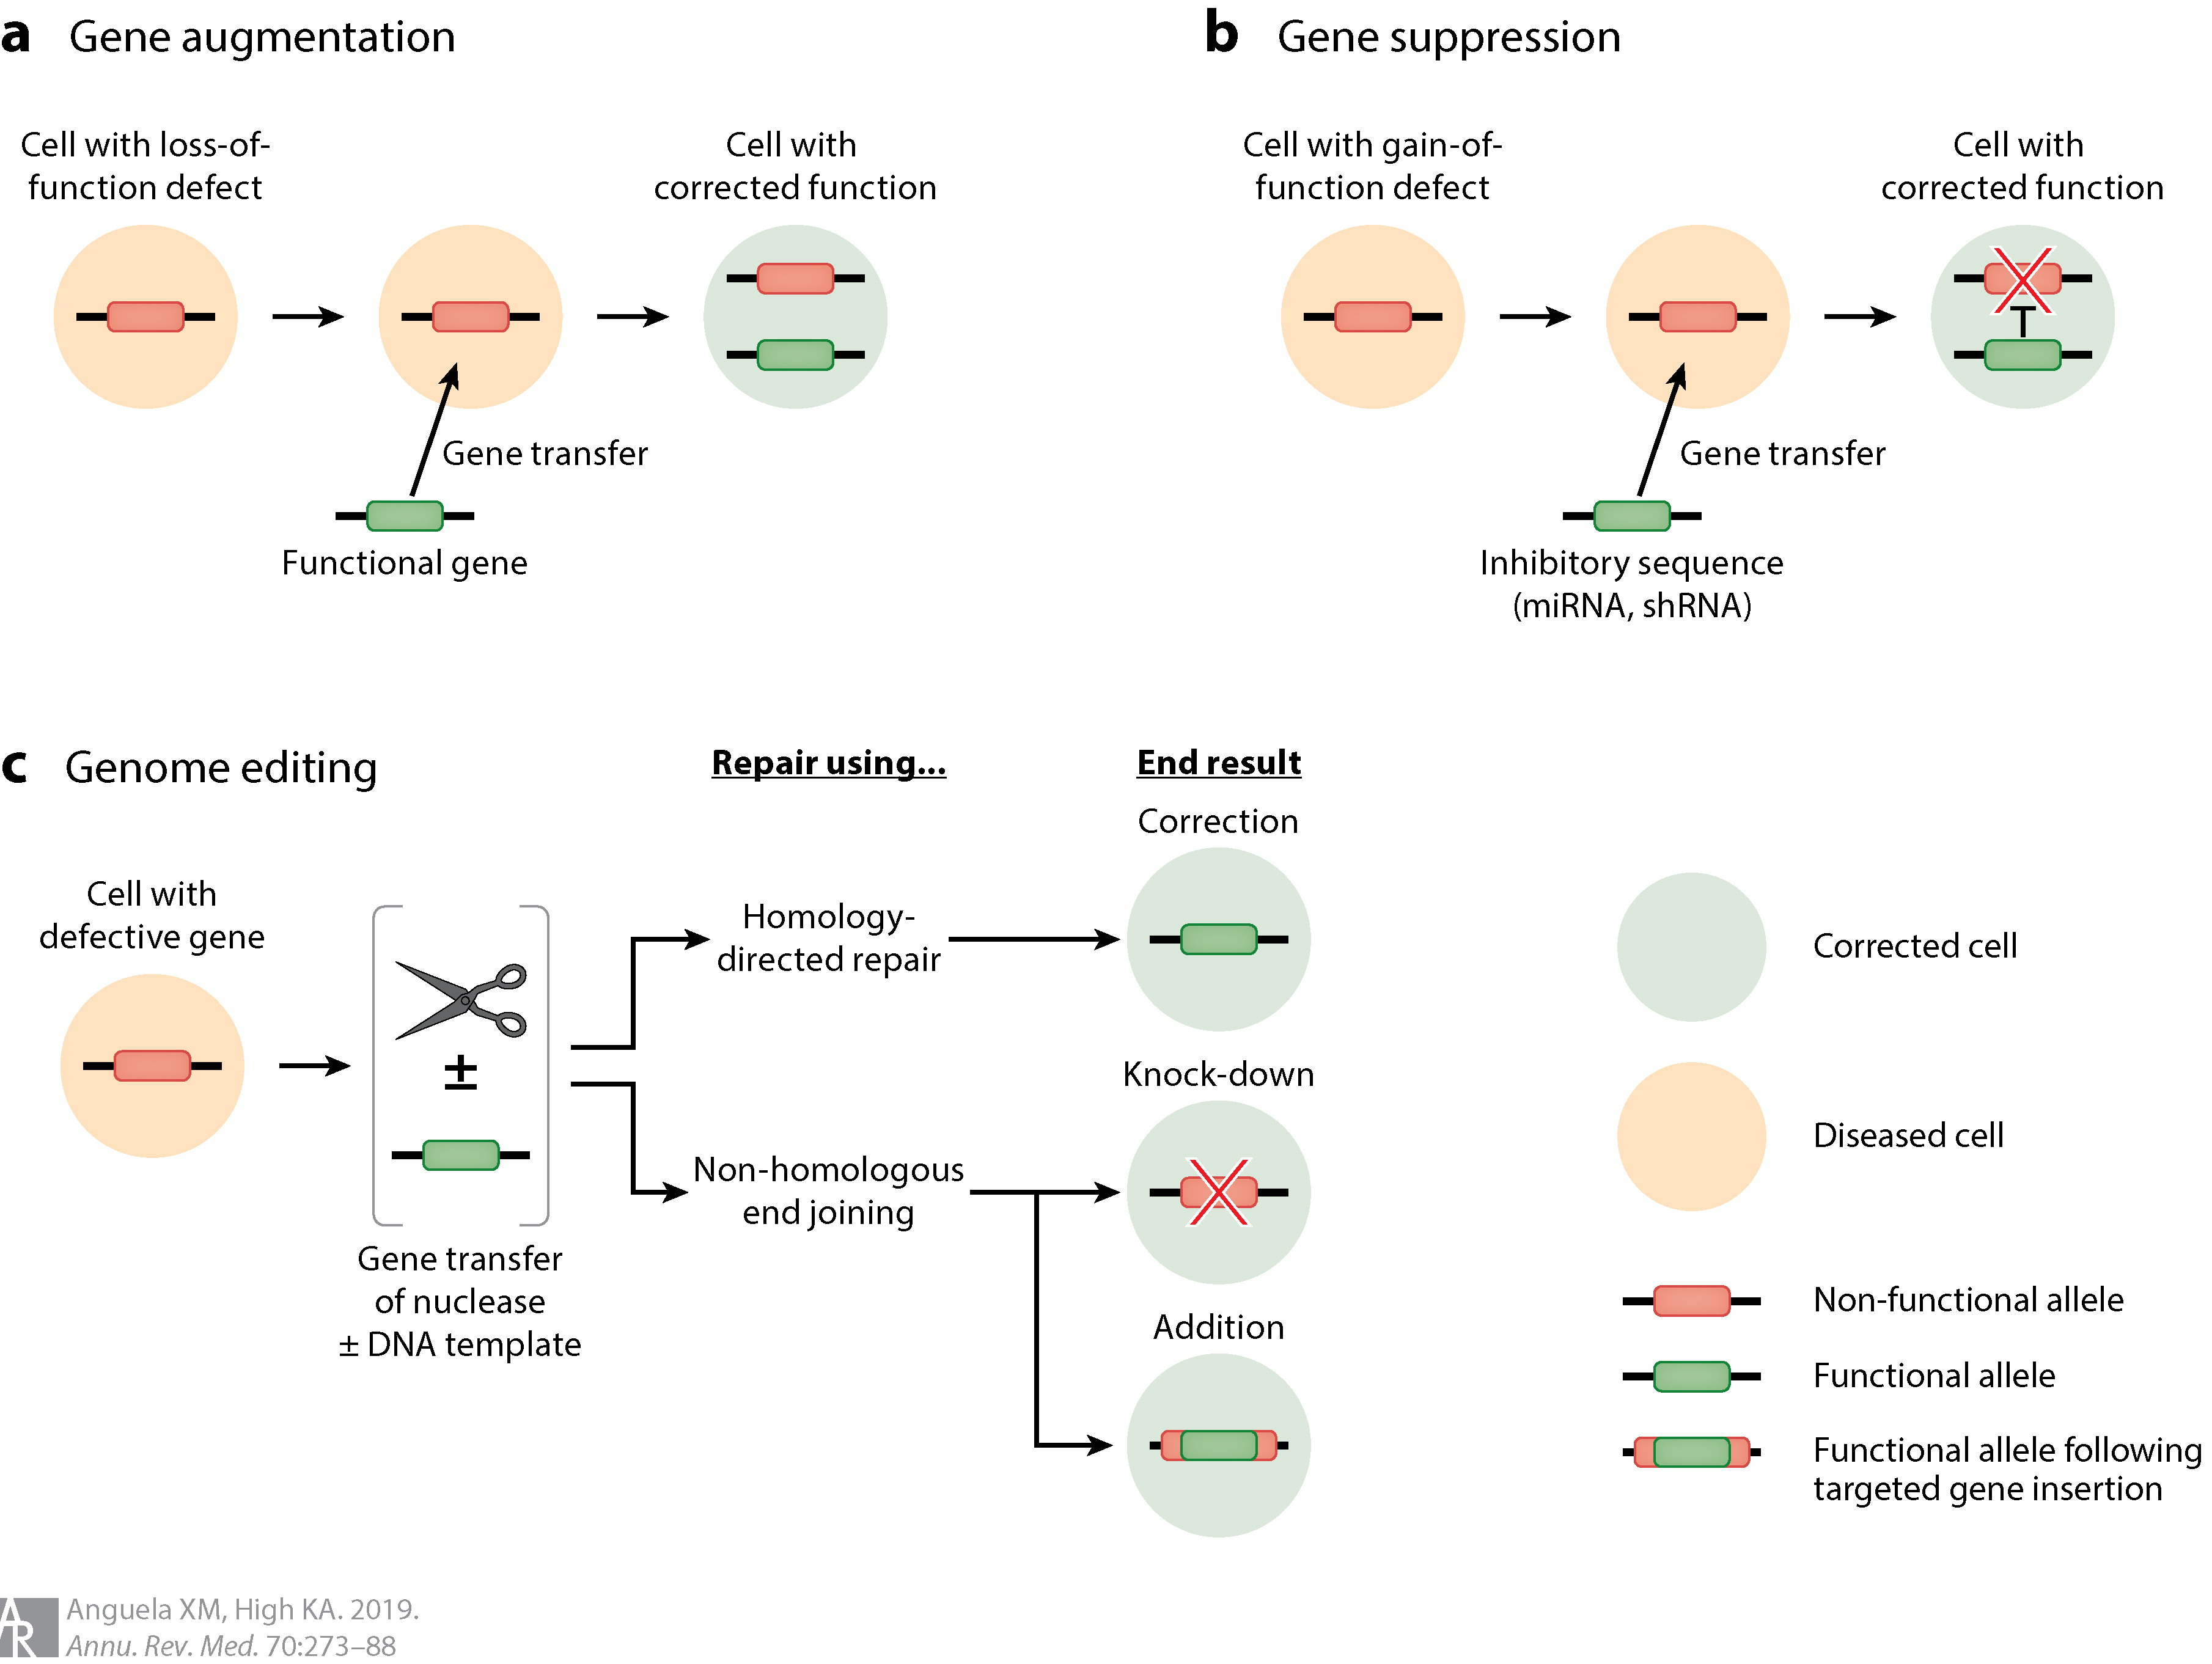
\includegraphics[width = 0.8\textwidth]{1introduction/pics/gene_therapy.jpeg}
\caption[Principles of gene therapy]{Principles of gene therapy. Reproduced from \citet{Anguela2019}.} \label{fig:gene_therapy}
\end{center}
\end{figure}

Augmentation gene therapy introduces an healthy gene copy to restore the normal functionalities of the protein of interest and thus of the cell: it usually consists in the delivery of a DNA strand, which in turn can be internalised in the genome and thus spread when the cell replicates, or not internalised and thus can influence the functionalities of the particular transfected cells only \citep{Anguela2019}.
%
Suppression gene therapy suppresses a detrimental gene, and this is particularly useful in the case of cancer, to impede cancer cells replication. Usually this strategy employs RNA interference, delivering miRNA (microRNA) or siRNA (small interfering RNA) strands which repress the transcription of the problematic RNA sequence.
%
Finally, gene-editing, the most recent advance in the field, overlooks the possibility of correcting base pairs mutations to restore the original healthy sequence, and is often done through the functionalisation of the CRISPR-Cas9 technology, a mechanism found in prokaryotic organism as defence against viruses \citep{Barrangou2015}:
%
CRISPR (clustered regularly interspaced short palindromic repeats) is a library of DNA fragments from viruses that have previously infected the prokaryote, and the Cas9 enzyme (CRISPR-associated protein 9) uses these sequences to recognize and cleave strands of DNA complementary to the CRISPR sequences to block subsequent infection preventing the viral replication. Research has been able to engineer the CRISPR-Cas9 technology to edit (rather than simply cleave) genes within eukaryotic organisms \citep{Zhang2014cas}, thus performing a therapeutic role.

Despite the challenges posed by the development of genome editing tools, and the risk associated to them (for example the possibility of deleterious insertional mutagenesis or deleterious immune responses), at present six gene therapies have received approval in the Western world \citep{Anguela2019}, with many more undergoing regulatory review. 

One of the main problems in the development of such therapies lies in the identification of a suitable vector: delivery of free genome in solution results in poor internalisation and low therapeutic effect.
%
Thus nowadays the outlook of gene therapy research lies not only in improving specific cargos, but also in the research of appropriate vectors with low toxicity, low induced immune response and high delivery efficiency. Viruses can be used, modifying their genome to include the necessary sequence and remove the ones promoting viral replication \citep{Naldini2011,Mingozzi2011}, but synthetic vectors are now investigated for a virus-free delivery strategy. The system studied in this thesis proposes, among its other functions, to deliver genetic material into human cells.


\section{Delivery of therapeutic material}
The problem of gene delivery sets a parallel with the small drug one, introduced at the beginning of the chapter. Indeed small molecules need delivering agents to be efficiently internalised in the cells, in the same manner that genes do.

To reach the aimed organ, therapeutic molecules must be compatible with the different cellular environments they cross, but be preferentially retained, and act only on the ones they are designed for. This implies a subtle balance between a invasive activity on one side, and mimesis on the other, to minimise the possibility that the compound is recognised as dangerous and disposed by the immune and reticuloendothelial systems.

As an example, one can think of the trip of a standard, orally administered drug, passing through the digestive system, with its challenging acidic environment and limited permeation across the intestinal epithelium, and from there to the blood stream \citep{Masaoka2006, Mitragotri2014}. 
%
At this point, the drug is generally coated by a protein corona based on its shape and charge \citep{Krol2012}. The nature of this coating is difficult to predict and can disrupt or decrease significantly the efficacy of a compound as it modifies the way it is recognised and absorbed.
%
From the blood the drug diffuses in the tissues flanking the blood vessels naturally depleting its concentration downstream \citep{Krol2012}, so that regions further away from the injection region have less chances of getting a sizeable dose. 
%
Moreover some specific tissues are highly impermeable: the blood brain barrier (BBB) for example allows the passage of small molecules with high lipid solubility only \citep{Pattni2015, Krol2012}; while tumoural tissues are instead poorly vasculated, reducing the chances of delivery at their interior \citep{Pattni2015}.

For all the above reasons, research has focused on developing systems to assist the delivery of drugs. A mimetic carrier can not only improve delivery, but also be designed to selectively bind to particular tissues, or to trigger the drug release after a delay, or only upon changes in environmental variables (for example pH) to reduce drug concentration in non targeted regions. A stand alone field of research has then focused on the development of delivery vehicles irrespective from the quest for new drugs. The optimised products of the two separate efforts can then be paired according to the condition to address, to give a successful therapy.

At present, many molecules have been successfully employed to build drug vehicles, both organic and inorganic, to offer a range of different physico-chemical characteristics useful to target different cells \citep{Hughes2005} (Figure \ref{fig:vehicles}). We briefly list them to point out the variety and exoticity of structures which are useful, sometimes unexpectedly, to the medical world, and we then focus on peptidic delivery vehicles: once more this class of molecules can offer a solution to a therapy-related task.

\paragraph{Inorganic materials for small drugs delivery}

%\begin{figure}
%\begin{center}
%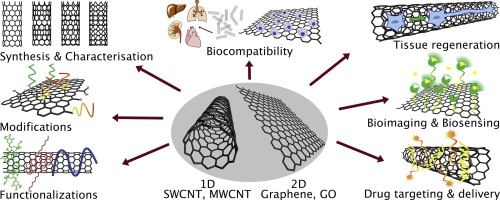
\includegraphics[width = 0.5\textwidth]{1introduction/pics/carbon_review.jpg}
%\vspace{0.2cm}
%\caption[Materials for drug delivery vehicles]{INCLUDE ONE EXAMPLE IMAGE (FROM PAPERS) FOR EACH MATERIAL (nanoparticles, carbon, polymers, lipids, DNA, proteins).} \label{fig:vehicles}
%\end{center}
%\end{figure}

Many inorganic compounds have been used to transport drugs or to enhance their biocompatibility. A first class is constituted by metal nanoparticles, with golden nanoparticles covering a major role. Thanks to their metallic nature, these materials can be customised in shape and size (down to a 10 nm radius), and possess optical properties that allow to track them inside the body or to thermally stimulate them to trigger drug release \citep{Boisselier2009}. They can also be coated with biologically active moieties to enhance their mimesis \citep{Singh2018}. For these reasons, they are used to selectively treat tumoural cells, but up to now only a few golden nanoparticle based compounds have made to the clinical stage, as there are mixed evidence about their toxicity \citep{Boisselier2009}. 

Similarly, materials made from carbon, especially carbon nanotubes, can be used for biomedical applications as they have a high loading efficiency thanks to the high surface area and easy interaction with biomolecules through van der Waals forces, $\pi$-$\pi$ stacking or hydrophobic effect \citep{Erol2017}. They can be conjugated to extra organic groups to increase their biocompatibility and have potential for targeted drug release upon change in environmental pH \citep{Depan2011}.

Finally polymers are a class of inorganic molecules already well validated as drug eccipients. The most notable example is Polyethylene glycol (PEG): thanks to its high hydrophilicity, it is widely used to coat structures (e.g.\ inorganic nanoparticles, peptides) which in turn carry a drug \citep{Lammers2009}; or as a stand alone carrier system with high drug payload \citep{Liechty2010}. The great strength of polymers is their flexibility: as each of their constituent monomers can be either hydrophilic or hydrophobic, they can be engineered to assemble in many different structures, to swell slowly in water triggering a sustained drug release \citep{Nicolas2013}, or to undergo sol-gel phase transition upon specific changes in the environment \citep{Liechty2010}.


\paragraph{Organic materials for delivery: lipids and DNA} \label{sec:organic}

A somehow opposite approach for designing drug vehicles consists in using molecules similar to the ones present in the body, such as lipids, DNA and peptides, in an effort to exploit already available biocompatible materials and reduce toxicity \citep{Yoo2011}.

A great variety of lipids is present in the cell membrane, and the chemical space is further enlarged by the production of synthetic ones. The components selected for drug delivery are usually taken from the biological lipidome, modifying the composition and possibly including synthetic molecules to tune the release and robustness to degradation \citep{Yingchoncharoen2016}.
%
Being amphiphatic, lipids can encapsulate efficiently both hydrophobic or hydrophilic drugs, arranging respectively in micelles (monolayer spheres with the hydrophobic tails facing the interior) or in liposomes (bilayer spheres with a water filled core) \citep{Bunker2016}, and by now, many lipids are approved as delivery agents for cancer and infection drugs \citep{Pattni2015paper, Jain2017}.

DNA scaffolds are instead a more novel tool: DNA origami is nowadays an established technique to build three dimensional customised solids \citep{Linko2015}, and the nanometric knowledge about their constituents allows to fine tune them for a triggered release of the content \citep{Douglas2012}. First studies proved them successful in delivering anticancer agents \citep{Zhang2014, Jiang2012}, however they are very sensitive to different cellular environments which challenge their stability. This, united with high production costs and the relative young developments in their manipulation, prevented them to constitute a viable class of carriers so far, but at the same time holds promise for future improvements and applications.


\subsection{Peptidic scaffolds} Another widely used and trustworthy mimetic vehicle comes, quite surprisingly, from the world of pathogens: viruses have co-evolved with humans, to be able to penetrate into cells where they complete their reproductive cycle \citep{Lobo2009}. Therefore their capsid, the peptidic shell encapsulating the viral genome, is highly suitable for cell penetration. The first application sought historically was to employ genome free viruses to stimulate and train the natural immune response against the respective genome-loaded ones, creating viral vaccines - in a concept similar to the inoculation of dead bacteria to counteract the infections caused from them \citep{Lauer2017}.
Later in the history, their potential as cargo carrier was pursued by first modifying the original genetic material to include sequences beneficial for the host cell, and inactivate the ones promoting the infectious duplication at the same time \citep{Daya2008}.
%
To fully exploit the potential of a peptidic carrier many efforts have focused on synthesising in vitro gene-free capsids, either as they appear in nature \citep{Wu2009} or designing artificial building blocks, which assemble in so called Virus-Like particles (VLPs) which trigger lower immune response.
%
Similarly to other delivery vehicles, the surface of VLPs can be functionalised with additional molecules to improve the target selectivity and increase biocompatibility, while the peptidic scaffold grants robustness to the structure. Therefore, VLPs loaded with drugs can be tuned for an efficient intra cellular release \citep{Ma2012}.

A step further in engineering peptidic structures is represented by the design of self-assembling functional blocks from first principles. Indeed, self-assembling peptides can form nanostructures ranging from nanoparticles to nanotubes, nanofibers, nanorods and hydrogels \citep{Fan2017}.
%
Among their advantages, peptides present biocompatibility and a tunable bioactivity thanks to their chemical diversity, which helps in tailor the assembly toward the target of interest \citep{Fan2017}. Moreover, the variety of amino acid available makes possible to load peptidic structures with both hydrophilic and hydrophobic drugs, according to their amino acid composition \citep{Ma2012}.
%
The peptidic self-assembly is modulated by the peptide length and its hydrophobic or hydrophilic character, given by its amino acid composition: simple phenylalanine dipeptides were designed with inspiration from a pathogenic pathway of molecular self-assembly and were shown to self-assemble in a multi-scale process producing nanotubes able to load drug molecules \citep{Silva2013}. The relatively small diphenylalanine building block is non the less complex as it bears two charged termini (as the process is observed at neutral pH), and two aromatic hydrophobic rings, so that the dipeptide is driven towards assembly by the hydrophobic forces acting on the phenylalanine side chains and the complementary charges of the termini.

In a different approach, longer sequences can be employed to guide the formation of the local structure, as they organise spatially in well studied secondary structures with known interactions among themselves.
%
This knowledge is possible as proteins are a fundamental component of the human body and as such an updated database of their structure is available (the Protein Data Bank \citep{PDB}) and can be queried to understand how small peptides hierarchically assemble into larger units.
%
Moreover, the vast literature on their interactions with membranes, cell receptors and in general biological components, can inspire the design of building blocks sensible to particular triggers within the body. From this background, the outlook of protein design often goes in the direction of surpassing natural limitations, synthesising exotic, non natural, geometries \citep{Yeates2019,Malay2019} for multifunctional materials.


\section{Closing the circle: an antimicrobial drug delivery vehicle}

Twice in this introduction peptide design has been brought to the reader's attention. First, it can produce antimicrobial peptides with improved potency or selectivity, or reduced toxicity. Second,  design can engineer self-assembling building blocks for the formation of delivery scaffolds. As design is not bound to natural rules, it can foresee and imagine multifunctional materials which are not observed in nature. In particular, the introduction above poses the question of whether it is possible to engineer peptides able to perform both an antimicrobial and a delivery function at once (either of drugs or genetic material).
%Thus, the relevance of such compound would be twofold.

Such self-assembling, antimicrobial compounds would have a twofold interest for medical applications.
%
First of all, self-assembly is functional to the antimicrobial activity: many AMP sequences have a weak potency, and only a high (critical) concentration can trigger the bactericidal mechanism. This is intuitive in the case of the carpet model strategy (see Section \ref{AMP_mechs}), where AMPs lay homogeneously on the surface of the bacterial membrane and breaks it upon sufficient coverage of its area. Also the barrel-stave and toroidal pore models rely on the mutual interactions between peptides to maintain the pore edges.
%
Generally, as AMPs are positively charged, the localised presence of many copies of a sequence enhances the local electric field and charge imbalance, which are critical to the membrane stability. 
%Thus a self-assembling sequence will enhance the local concentration which is crucial to initiate the membrane disruption.
%
Second, in order for the assembly to be able to perform the additional delivery function, it must be able to either organise in a tailored structure (for example a capsule able to host a drug), rather than an amorphous aggregate, or to co-assemble with the cargo of interest.

Out of all the possible applications, the most promising is perhaps the use of such vehicles to deliver drugs to treat metabolic or genetic diseases: while the cargo tackles a defect of the host system, the vehicle can counteract the proliferation of bacteria. This is particularly important in situation where the host immune response is weakened and thus infections normally harmless can spread and cause damage.
%
However, it must be noticed that the cargo is not bound to be a small molecule, as long as it can effectively co-assemble with the peptidic carrier. As mentioned in the previous section, gene therapy is also an actively expanding field which looks with interested at the development of vehicles for genetic material. Given that viruses have been the first choice for DNA/RNA delivery so far, peptidic carriers seem a natural evolution of them.

\bigskip
Given the above premises, it is evident the importance of pursuing the research on novel multifunctional peptidic materials.
As mentioned when discussing AMPs design, to understand such systems, each of them must be characterised by itself, as a generalised knowledge is still lacking.
With this aim, this thesis proposes to elucidate the behaviour of a specific synthetic self-assembling peptide, suitable for antimicrobial activity and gene delivery strategies. Its full characterisation will complete the knowledge on its mechanisms of action and complement the broader information already known on the class of such functional building blocks. This will be crucial to engineer new synthetic blocks with improved characteristics, either regard their antimicrobial activity, assembly performances, or tailored cargo delivery.


\subsection{Capzip} \label{sec:capzip}

\begin{figure}
\begin{center}
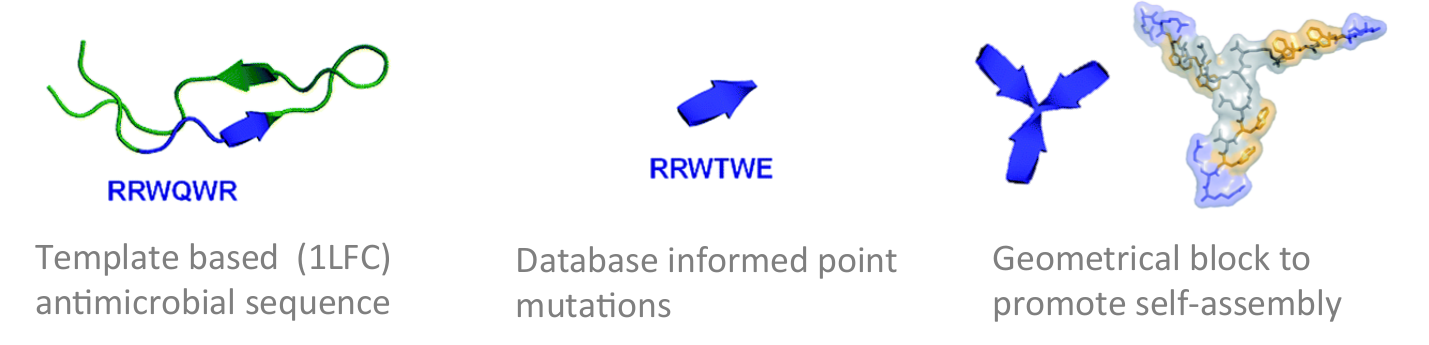
\includegraphics[width = \textwidth]{1introduction/pics/capzip.png}
\caption[Cazip molecule]{Capzip molecule scheme and bond representation. [TO BE IMPROVED] Adapted from \citep{Castelletto2016}.} \label{fig:capzip}
\end{center}
\end{figure}

The molecule capzip has been designed to perform the functions mentioned above at once. To recapitulate, the properties it possesses are:
\begin{enumerate}
\item assembly into nanoscale virus-like capsules with and without nucleic acids. This ensures that the vector can autonomously form and thus there is flexibility in the choice of the cargo;
\item antimicrobial activity of the molecule itself and of the capsule on a time scale useful for therapeutic applications;
\item promotion of gene transfer into mammalian cells when the peptide is co-assembled with the RNA strands, without causing cytotoxic and haemolytic effects.
\end{enumerate}
%
Furthermore, the design effort aimed at building a template structure of minimal complexity, in order to reduce the synthesis effort to a short sequence. Arguably, short sequences are also more flexible in their assembly: it is thus important to explore them and prove whether even small blocks can form ordered structures.

Based on the above requirements, two design principles emerged: first the employment of a non-linear structure. There is indeed some evidence suggesting that non linear peptides are more prone to assemble in three dimensional structures, opposed to planar ones \citep{???}, and this holds in particular for short sequences which do not fold into a defined secondary structure.
%
The second principle consists in the use of a template antimicrobial sequence which is short and has proved potency.
%
Given that AMPs are usually anionic, the co-assembly with anionic RNA sequences is arguably inherited by consequence.

To satisfy the above guidelines, a short peptidic scaffold constituted by a $\beta$-Alanine and two Lysins has been engineered.
%
Three identical copies of the antimicrobial sequence of choice are covalently bonded to the N-terminus of the scaffold sequence and to the nitrogen atom of the Lysin residues side chains (Figure \ref{fig:capzip}).
%
Regarding the antimicrobial sequence selected, it has been derived from the antimicrobial peptide bovine lactoferricin, which is in turn a portion of the Lactoferrin protein.

\paragraph{Lactoferrin} Lactoferrin is an iron binding protein present in milk (in which it is most abundant, hence its name), saliva and other secretions, as well as in polymorphonuclear leukocytes.
%
It works as an iron binder and provides a natural defence against bacteria and fungi \citep{Sanchez1992,Arnold1977,Arnold1980,Kirkpatrick1971,Jahani2015}, constituting a first defence for infants.

Lactoferrin contributes to bacterial suppression in several ways. At present, its known modes of action fall in three categories: first, thanks to its iron sequestering capabilities, it removes essential substrate required for bacterial growth \citep{Farnaud2003}; second, it interacts with bacterial membranes and in particular binds to the lipopolysaccharides of bacterial walls, oxidising them and affecting the membrane permeability with consequent cell lysis \citep{Farnaud2003}; finally it is implicated in the stimulation of different immunological cells (killer cells \citep{Shau1992}, polymorphonuclear leukocytes, and macrophages \citep{Gahr1991}).
The peptide fragment responsible for binding of lactoferrin to the bacterial membrane, named lactoferricin (Lfcin), has been identified near its N-terminus and found to have a more potent bactericidal effect than intact lactoferrin on a wide range of bacteria \citep{Gifford2005,Bellamy1992,Tomita1994,Wakabayashi1996}.
%
Similarly, a synthetic short peptide derived from a subsequence of human lactoferricin has been proven effective against bacteria as it depolarises the cytoplasmic membrane decreasing the pH gradient \citep{Aguilera1999}.

The bovine homolog of lactoferricin (LfcinB) has a higher bactericidal potency than human lactoferricin on several bacteria \citep{Cochran2001} and therefore has been more extensively studied. Its active core LFC is a 25-amino acid sequence which adopts a helical conformation in the full structure but, once isolated, crystallises in a $\beta$-hairpin with a disulfite bridge nearby the terminals which stabilises the fold, but was shown to be not essential for bactericidal activity \citep{Cochran2001}.
%
Further experiments on LfcinB subsequences identified an even shorter antimicrobial core, constituted by the six amino acids RRWQWR \citep{Schibli1999}. This core presents a characteristic Tryptophan zipper motif WTW, which appears very often in nature in $\beta$-turn and $\beta$-sheet conformations, paired to another copy of the same motif, so that Tryptophan rings from facing strands are packed tightly against each other in an alternated way \citep{Cochran2001} (Figure --).
In general, the six amino acid sequence contains both charged and hydrophobic residues, in line with the usual composition of antimicrobial peptides. Accordingly, its antimicrobial action is likely derived from the interaction with biological membranes through charge recognition first and aromatic rings insertion in a second moment.

To further elucidate this mechanism, several experimental investigations have been carried both on LfcinB and its subsequences. First, the structure of LfcinB in solution has been investigated by NMR (Nuclear Magnetic Resonance), resulting very flexible \citep{Hwang1998}. Then, the binding of its antimicrobial core to sodium dodecyl-sulfate micelles was studied \citep{Schibli1999}, suggesting a favourable interaction of aromatic residues with the micelles surface.
%
Similar experiments were performed on large unilamellar vesicles, constituted by lipids modelling biological membranes: ePE:ePC was chosen as a model of a mammal membrane, and ePE:ePG or ePC:ePG for a bacterial one. The experiments showed preferential binding to the latter ones, based on Tryptophan fluorescence \citep{Nguyen2005}, suggesting a selective antimicrobial action on anionic membranes.
%
Additional experiments have been performed on the full sequence or mutated subsequences \citep{Tsutsumi2012,Arseneault2010} to investigate the binding to other different model membranes but, as the systems investigated are slightly different, as well as the experimental conditions, therefore it is difficult to relate them and give a unified interpretation of the modes of action of lactoferricin derived peptides.

Finally, an alanine scanning has attempted to clarify the role of each amino acid in the antimicrobial activity of the LFC peptide \citep{Strom2002}. The results suggested a binding function for the Tryptophan residues, in line with one of the roles Tryptophan can assume in antimicrobial peptides \citep{Chan2006}. Other possible roles involve its propensity to form hydrogen bonds, in which case the residue would position itself at the interface between solution and membrane, rather than inside the latter (which happens instead when Tryptophan residues have a binding role).

\paragraph{The designed block}
From the active core of LFC (of sequence RRWQWR), a mutated sequence was obtained to comply the design criteria of a self-assembling building block. Two mutations were introduced to favour the assembly of arms belonging to different molecules in an antiparallel fashion. Specifically, given that the original RRWQWR sequence is found in a $\beta$-sheet (at least in the crystal lattice), the mutations aim at promoting a similar structure. Therefore, the Glutamine residue and the C-terminal Arginine of the lactoferrin motif were replaced with Threonine and Glutammic acid residues to have a self-complementary sequence RRWTWE: the pairing is promoted by the attraction of opposite charges at the ends of the sequence.
%
Three copies of this sequence were thus covalently bonded to the scaffold described previously and shown in Figure \ref{fig:capzip}, to obtain a self-assembling molecule in a three dimensional shape, hosting multiple copies of an actively antibacterial sequence.

%With the virus architecture adopting an n-fold rotational symmetry, where n is usually 3 or 5 or both,9 a triskel conjugate of RRWTWE was generated to give a self-assembling motif with a trilateral symmetry reminiscent of native cage-like subunits (Fig. 1b–e and S1 in ESI†).

\subsection{A viable systems: experimental background and question}
Many experiments have been performed to verify that capzip had the characteristics it was designed for. The set of experimental results obtained on the molecule has been published in Reference \citep{Castelletto2016}, while more recent results extend and consolidate the previous findings.

\begin{figure}
\begin{center}
\textbf{AFM/TEM \ \ \ \ \ \ \ \ \ \ \ \ \ \ cryo-em}
%\subcaption{}\label{fig:exp_capzip_a}
%\subcaption{} \label{fig:exp_capzip_b}
\bigskip

\textbf{fluo hollow capsule \ \ \ \ \ \ \ fluo RNA uptake}
%\subcaption{} \label{fig:exp_capzip_c}
%\subcaption{} \label{fig:exp_capzip_d}
\caption[Experimental results on capzip]{... Reproduced from \citep{Castelletto2016}} \label{fig:exp_capzip}
\end{center}
\end{figure}

\paragraph{Experimental results} First, the assembly ability have been tested: the peptide does not show assembly in pure water (as verified by Dynamic Light Scattering), while in biological buffer (MOPS, 150 mM) at physiological pH of 7.0 it forms capsules with dominating size range of 20-200 nm. This is confirmed by images of the capsules obtained with multiple techniques, namely transmission electron microscopy (TEM) (Figure \ref{fig:exp_capzip}), atomic force microscopy (AFM), and cryo-scanning electron microscopy (SEM).
%
The fine structure of these assemblies appears irregular to the resolution power of such techniques. Some insight into the details of the assembly is given by Circular Dichroism (CD) spectra, which show a profile characteristic of $\beta$-turns and contain elements of a $\beta$-sheet structure and of indole rings, with minima at $\lambda \sim$ 200 nm and 214 nm.
%
Complementary evidence about the overall shape of the assembly was provided by the cross-sectional analysis of the assembled capsules by fluorescence microscopy using fluorescein to label capzip. The signal comes from the wall of the capsule only, showing an inner cavity (Figure \ref{fig:exp_capzip}).
%
Finally, small angle X-ray scattering (SAXS) measurements were consistent with compact capsules interfacing with solvent.

The assembly process is also tested and monitored in combination with small interfering RNAs (siRNA): as mentioned in section \ref{sec:gene_th}, these sequences are a promising tools for RNA interference techniques which aim at inhibiting the expression of specific genes, however, they are easily degradable and thus difficult to deliver to the target cell without an appropriate vehicle.
%
The co-assembly of a 21 base pairs duplex with the peptide shows the formation of structures similar to the ones formed by the stand alone peptide only: CD spectra highlight the helical signal from RNA together with the features proper of the peptide.

These co-assembled structures were tested for siRNA delivery in HeLa cells, showing that the presence of the peptide favours the internalisation of the genetic material with respect to the transfection results of a pure siRNA control. The delivery of fluorescent siRNA (Figure \ref{fig:exp_capzip}) showed that the internalisation occurred within the first hours from the transfection in localised regions of the cytoplasm, suggesting an endocytic uptake. This distribution was stable over the first five hours of incubation after which the fluorescence signal decayed.
%
Flow cytometry assays quantified the increase in siRNA uptake levels due to the presence of capzip, confirming that this molecule is competitive with other commercial transfection reagents (like Lipofectamine\textsuperscript{\textregistered}, unpublished results).

To further quantify the level of RNA internalisation, a mRNA knockdown experiment was performed on a HeLa cell line with two housekeeping genes, ACTB ($\beta$-actin, targeted) and GAPDH (reference) \citep{Crombez2009}.
%
The silencing of $\beta$-actin mRNA was detected 22 $\pm$ 2 hours after transfection; and its knockdown ``fitness" was expressed relative to cells treated with siRNA alone (background) and normalised against viable cell counts (Figure \ref{fig:exp_capzip}). Capzip fitness was lower than Lipofectamine\textsuperscript{\textregistered} one, however cells treated with capzip remained viable after 24 or 48 hour, resulting in higher cell counts than the samples treated with the commercial reagent, suggesting that capzip has little cytotoxicity.
%
The experiment above was performed at neutral to positive charge ratio close to one (where each siRNA molecule has a -42$\, e$ charge and capzip a +6$\, e$ charge), as test experiments performed at higher peptide-to-siRNA ratio showed no improved uptake.

Finally, the peptide does exert an antimicrobial function: the non-assembled peptide has shown to be effective against both Gram positive and negative bacteria (E. coli, P. aeruginosa and S. aureus), with no haemolytic effects and minimum inhibitory concentrations typical of other antimicrobial agents.
%
On Supported Lipid Bilayer with negative total charge (mixed DLPC and DLPG, 3:1 ratio), the capsules create localized pores within minutes, as proven by AFM experiments repeated in time. The pore depth ranges between 1.4 and 2.2 nm, which is smaller than the radii of the capsules, however it is sufficient to disrupt the structure of the membrane.
%
Finally, to prove the viability of capzip as antimicrobial agent in vivo, it was used to counteract methicillin-resistant S. aureus (MRSA) infections in G. mellonella larvae. The particular bacterial strain used was susceptible to vancomycin, which could be used as control: the larvae treated with capzip showed survival rates significantly higher than the untreated control, and comparable to those treated with high doses of vancomycin (unpublished results).

%MANCA: microfluidic results

\paragraph{Open questions} Despite the success of the experiments mentioned above, there is much information still to be uncovered on the precise mechanism of action of such peptide. 

Specifically, both the assembly process and the antimicrobial mechanisms contain some unknown: regarding the former, it is important to understand which amino acids or sub-structures allow the pairing of molecules, whether such pairing is specific or not, how reversible it is, and how rigid the final structure is.
%
Regarding the latter, it must be highlighted what molecules in the membrane the peptide binds to, and how this binding affects the full membrane structure. Finally, as there is evidence that the assembled molecule is a more powerful antimicrobial compound than the single molecule, it is interesting to understand whether any cooperative action is taking place or the enhanced antimicrobial power of the assembly is due only to the localised higher concentration.

Even if further experiments or future improvements in the techniques already employed might tackle some of the aspects above in a near future, arguably no experimental outcome can provide an atom-by-atom knowledge of the processes of interest in any time soon. Ideally though, one would like to track each of them, i.e. the processes happening in any the environments capzip has been exposed to (physiological solution, supported lipid bilayers, bacterial extracellular matrix, mammal cell membrane and cytoplasm) both in space and time with the finest level of details, and the impossibility of that leaves large gaps in the understanding of the system.


\section{A computational approach to understand capzip}

The gaps mentioned in the characterisation of the systems prompts for new investigations in order to complement the knowledge already provided.

Beside the quest to enrich the fundamental knowledge on self-assembling peptides and antimicrobial ones, the understanding of this very system is crucial for its further development. We outlined already in Section \ref{sec:amp_design} how antimicrobial peptide design can proceed from already viable templates and empirical principles, when first principles are not available. Similar rules hold for designing self-assembling peptidic materials, to obtained tailored delivery vehicles (see Section \ref{sec:organic}).
%
Therefore, a full knowledge of the interactions between peptides and between their assembled structures and the membrane, i.e.\ of the mechanism of its functions, will drive the engineering of new likewise peptides. A knowledge-driven design would hopefully provide new blocks suitable for a double action as the one capzip performs, and this in a shorter amount of time than a research based on less information or on a trial-and-error procedure of mutations in the chemical composition or in the architecture of the molecule. A few examples of possible knowledge-related improvements include the following:
\begin{itemize}
\item the knowledge of capzip binding mode to the bacterial membrane might suggest its suitability as a broad range spectrum compound or the possibility of tuning its action against specific pathogens;
\item understanding the molecule-molecule interactions classifies the robustness of the assembled structure and the possibility of designing block which disrupts under particular chemical conditions only;
\item querying the electrostatic profile of the assembled structure suggests which type of molecules, other than siRNA, could be efficiently co-assembled and thus delivered.
\end{itemize}

In recent years, computational techniques are becoming increasingly accessible and sophisticated and can usefully complement the incomplete experimental knowledge to give more insights into how biological systems work. For this reason, it seems natural to query such techniques to study the capzip system as well. Zooming into the details of the interactions can be performed via a theoretical modelling of the system in time, and thus through the simulation of its evolution, starting from few basic principles and the knowledge of the chemical composition of its parts. The technique this work focuses on is Molecular Dynamics simulations, which aims at reproducing the behaviour of a system of atoms in a semi-classical description using basic physical laws, as it will be described in details in the next chapter.

Thus it is the aim of this thesis to prove that Molecular Dynamics simulations can clarify further details on the assembly mechanisms of capzip and on its interactions with biological membranes, in order to gather more information on the system and contribute in the future to the designed of new molecules with enhanced functional capabilities.

%MORE SPECIFIC QUESTIONS

%\paragraph{Bits}

%In the triskel conjugate, RRWTWE is prone to fold as a b-turn and pair into a b-sheet with another arm of another conjugate.7 Triskelions are then
%compact globular morphology of the capsules observed by AFM in solution (Fig. S3†). 

%The specificity of these antibiotics allows generally to selectively target the desire species of bacteria, however it has the drawback that small modification in the target can easily invalidate the effect of the drug. 

%The typical time at which this resilient population appears varies greatly according to the mechanism targeted by the drug, but also and especially by how this is administered, resulting in the modern ways of treating infections a particularly fertile ground to train drug-resistant bacteria. Key reasons of the acceleration of the mechanism are the more extensive - and sometimes unjustified - use of antibiotics, both in the doses used for patients and in the world wide coverage that nowadays can, luckily, been reached. It must not be forgotten that a large portion, if not the majority, of antibiotics do not come from human treatments but actually from agriculture and breeding.
%
%This increased pressure allow for a fast spread of resistance, but the emergency comes from the parallel lack of new discoveries of novel drugs. The few discovered and approve are kept as last resources and used carefully, both to prevent insurgence of resistance as long as possible and for their collateral effects: indeed, the inefficacy of other drugs has pushed pharmaceutical industry to resort to compounds discarded in the first screening because too toxic for the human body.

%The design of new synthetic AMPs can enhance the self-assembly property to improve the antimicrobial activity and to tailor the final structure into an organized geometry suitable as delivery vehicle \citep{Wei2017, King2014, Norn2016, Korendovych2010, Vauthey2002}.
%The design procedure must necessarily be directed by means of both experimental and theoretical modelling techniques \citep{Fjell2011, Maccari2013, Zhang2015}. Indeed, in silico techniques help to evaluate the physico-chemical characteristics of novel compounds and select the sequences suitable for the purpose. Additionally, they can elucidate the mode of actions of the antimicrobial activity which is still unclear for many AMPs, despite the vast body of experiments performed in the field \citep{Nguyen2011, Chan2006, Ulmschneider2017},

%In this context we want to employ computational techniques to investigate the characteristics of a synthetic antimicrobial peptide designed and tested for its self-assembly characteristics. Capzip \citep{Castelletto2016} is a branched peptide which incorporates three copies of a six amino acids AM sequences (one for each branch, SI Figure \ref{fig:SI_capzip_formula}).
%The sequence (RRWTWE) is a mutation of the antimicrobial region RRWQWR of the bovine lactoferricin peptide (PDB entry 1LFC)\citep{Schibli1999}. The mutations have been introduced to create a self-complementary sequence prone to antiparallel $\beta$-sheet formation with other identical sequences belonging to different molecules, via pairing of opposite charges \citep{Castelletto2016}. The three branches enforce a 3-fold rotational symmetry, reminiscent of the architecture of viral subunits, which aims at generating a three dimensional self-assembling motif, as the branches lies onto different planes.

%One of the key advantages of AMPs over pharmaceutical antibiotics is the ability of some of these peptides to also modulate immune responses. For example, in addition to their direct antimicrobial activity, AMPs can protect the host by a range of mechanisms: chemotactic activity, attracting leukocytes; modulation of host-cell responsiveness to TLR ligands; stimulation of angiogenesi enhancement of leukocyte/monocyte activation and differentiation; and modulation of the expression of proinfl ammatory cytokines/chemokines (Figure 1). For example, LL37 has been shown to attract neutrophils, monocytes, mast cells and T cells. Different groups of AMPs appear to have distinct chemotactic activities from each other. 
%Indeed, a common feature across most of them is the targeting of the bacterial membrane, generally in an unspecific way: membranes of different bacteria share often common characteristics, with all their species classifiable in two groups (Gram positive or negative) according to their membrane(s) structure, and thus AMPs are often effective on many representative of one class, if not both.

%Modification of AMPs with Covalent Bonds,  Modification of AMPs by Changing Amino Acid Content, Modification of AMPs by Amidation, Modification of AMPs with Unnatural Amino Acids, Modification of AMPs with Computer-Assisted Methods, New AMP Design by Homology Modeling

%torres: determining structure-activity relationships. site-directed mutagenesis, computationaldesign approaches, synthetic libraries, template-assisted methodologies, and mechanism-based strat-egies. 

%Gandhi2014 for nanocarrier for siRNA/miRNA

%Joo2016 Andersson2016 AMR to AMPs

%approved peptidic drugs Usmani2017 they are 884
%Recent advances cell-penetrating peptide-assisted drug delivery Langel2015
%Designing improved active peptides for therapeutic approaches against infectious diseases Gomes2018 READ

%Molecular mechanisms of membrane targeting antibiotics Epand2016 READ
%BASIS FOR SELECTIVITY OF CATIONIC ANTIMICROBIAL PEPTIDES FOR BACTERIAL VS MAMMALIAN MEMBRANES 2005Glukhov
%The therapeutic applications of antimicrobial peptides (AMPs): a patent review Kang2017
